%% LyX 2.0.5.1 created this file.  For more info, see http://www.lyx.org/.
%% Do not edit unless you really know what you are doing.
\documentclass[10pt,twocolumn,english]{svjour3}
\usepackage[T1]{fontenc}
\usepackage[latin9]{inputenc}
\usepackage{babel}
\usepackage{amstext}
\usepackage{amsmath}
\usepackage{amssymb}
\usepackage{graphicx}
\usepackage{bm}
\usepackage{esint}
\usepackage[authoryear]{natbib}
\usepackage[unicode=true,hidelinks]{hyperref}
\usepackage{subfig}

\newcommand{\argmin}{\operatorname*{arg\,min}}
\newcommand{\argmax}{\operatorname*{arg\,max}}
\newcommand{\erfi}{\operatorname{erfi}}
\newcommand{\psf}{\operatorname{PSF}}
\newcommand{\snr}{\operatorname{SNR}}
\newcommand{\var}{\operatorname{Var}}
\newcommand{\intRR}{\int_{\mathbb{R}^2}}

\makeatletter
%%%%%%%%%%%%%%%%%%%%%%%%%%%%%% User specified LaTeX commands.
\date{}

\makeatother

\begin{document}

\title{SimpleSTORM - a Fast, Self-Calibrating Reconstruction Algorithm for
Localization Microscopy}


\author{Ullrich K{\"o}the* \and Frank Herrmannsd{\"o}rfer* \and Ilia Kats \and Fred~A.~Hamprecht}
\institute{* contributed equally\\%
The authors are with the Multi-Dimensional Image Processing Group, University of Heidelberg, Speyerer Strasse 6, 69115 Heidelberg, Germany\\%
\email{ullrich.koethe@iwr.uni-heidelberg.de}}

\authorrunning{K{\"o}the, Herrmannsd{\"o}rfer, Kats and Hamprecht}
\titlerunning{SimpleSTORM}

\maketitle

\begin{abstract}
Although there are many reconstruction algorithms for localization microscopy, their use is hampered by the difficulty to adjust a possibly large number of parameters correctly. We propose SimpleSTORM, an algorithm that determines appropriate parameter settings directly from the data in an initial self-calibration phase. The algorithm is based on a carefully designed yet simple model of the image acquisition process which allows us to standardize each image such that the background has zero mean and unit variance. This standardization makes it possible to detect spots by a true statistical test (instead of hand-tuned thresholds) and to de-noise the images with an efficient matched filter. By reducing the strength of the matched filter, SimpleSTORM also performs reasonably on data with high spot density, trading off localization accuracy for improved detection performance. Extensive validation experiments on the ISBI Localization Challenge Dataset, as well as real image reconstructions, demonstrate the good performance of our algorithm. 
\keywords{localization microscopy \and STORM reconstruction \and matched filter \and noise normalization \and self-calibration}
\end{abstract}

\section{Introduction}

Localization microscopy techniques such as STORM and PALM have become
major tools for cell biology \citep{bates_08_super-resolution,heilemann_10_fluorescence,henriques_09_palm-and-storm,huang_10_super-resolution}.
Despite differences in the experimental procedures, these techniques
rest on a unified computational principle: Super-resolution images
are constructed by means of subpixel-accurate spot detection in a
sequence of images that was taken at optical resolution. Various algorithms
have been proposed for this task and many of them are available in
open-source software. We will briefly review related work in section \ref{sec:related-work}.

While many of these algorithms are able to obtain good
reconstructions in principle, their practical success requires a careful adjustment of
various configuration settings. This parameter tuning may be difficult
even for experts and raises the entry barrier for localization microscopy
novices. To overcome this problem, SimpleSTORM was designed to determine
all necessary parameters automatically from the raw image data
during an initial \emph{self-calibration phase} that precedes the
actual reconstruction phase. It can thus produce good reconstructions
with minimal user input, while still allowing optional configuration
by experts for non-standard use cases.

SimpleSTORM is based on an accurate model of the image acquisition
process. It assumes that Poisson-distributed photon counting noise is 
the dominant noise source. However, we explicitly account for the fact that photon counts
are only observed after a number of transformations by amplification
stages and digitization. In the assumption that the combined transformation
can be described by a linear equation, we can recover Poisson-distributed intensities
by inverting this linear equation after robust estimation of its parameters (gain and offset). Furthermore, we assume
that the point spread function (PSF) is fixed throughout the image sequence and 
can be determined as a non-parametric or parametric (Gaussian) model. 
Finally, we assume that the background intensity varies
at a much coarser scale than the PSF width and that less than half of the
pixels in any sufficiently large window contain signal. Under these
assumptions, the model parameters (gain and offset, PSF width, local
background intensity) can be estimated automatically in a self-calibration
and preprocessing phase.

In the reconstruction phase, the model parameters are used to transform
each frame such that it can be considered as a sum of a background-free
fluorescence signal and additive Gaussian noise with zero mean and
unit variance. Fluorescence spots can thus be recognized by a simple
statistical test: A pixel whose intensity is higher than three times
the noise standard deviation contains signal with a probability of
about 99.7\% (the threshold of the test can be adjusted to control
the detection sensitivity of our algorithm). Since the PSF spreads
over several pixels, whereas the noise of neighboring pixels is independent,
it is even more unlikely that three adjacent pixels exceed the threshold
just by chance. The combination of both criteria defines a reliable
mask for spot detection. Pixels under (and near) the mask are finally
convolved with a matched filter (i.e. a Gaussian filter corresponding
to the PSF) for optimal noise reduction and interpolated to the desired
resolution using a cubic spline. The coordinates of local intensity
maxima after interpolation are reported as the detected spots.

Specifically, our algorithm proceeds in these steps:
\begin{enumerate}
\item Robust estimation of the gain and offset parameters
\item Estimation of the width of a Gaussian PSF via the power spectrum
\item Linear intensity transform into unit gain and zero offset to make
the noise approximately Poisson distributed 
\item Anscombe transform of the intensities to make the noise approximately
normal
\item Dynamic background estimation and subtraction
\item Statistical test to determine the detection mask according to the
specified sensitivity
\item Matched filtering with the PSF for optimal noise reduction
\item Cubic spline interpolation to specified subpixel accuracy and maxima
detection
\end{enumerate}
On a standard laptop, our algorithm is able to process about 20 frames
per second for a typical raw image size of 200x200 pixels. It performed
favorably in the recent ISBI Localization Microscopy Challenge (\href{http://bigwww.epfl.ch/smlm/challenge/}{bigwww.epfl.ch/smlm/challenge/})
that carefully tested more than 20 reconstruction algorithms. In particular,
SimpleSTORM achieved high localization accuracy on high-density data,
where a relatively large number of spots was simultaneously switched
on in order to minimize total acquisition time. Software for our algorithm
is freely available in an easy-to-use GUI program.\footnote{\href{https://github.com/ukoethe/simple-STORM}{github.com/ukoethe/simple-STORM}}
\begin{figure*}
\begin{centering}
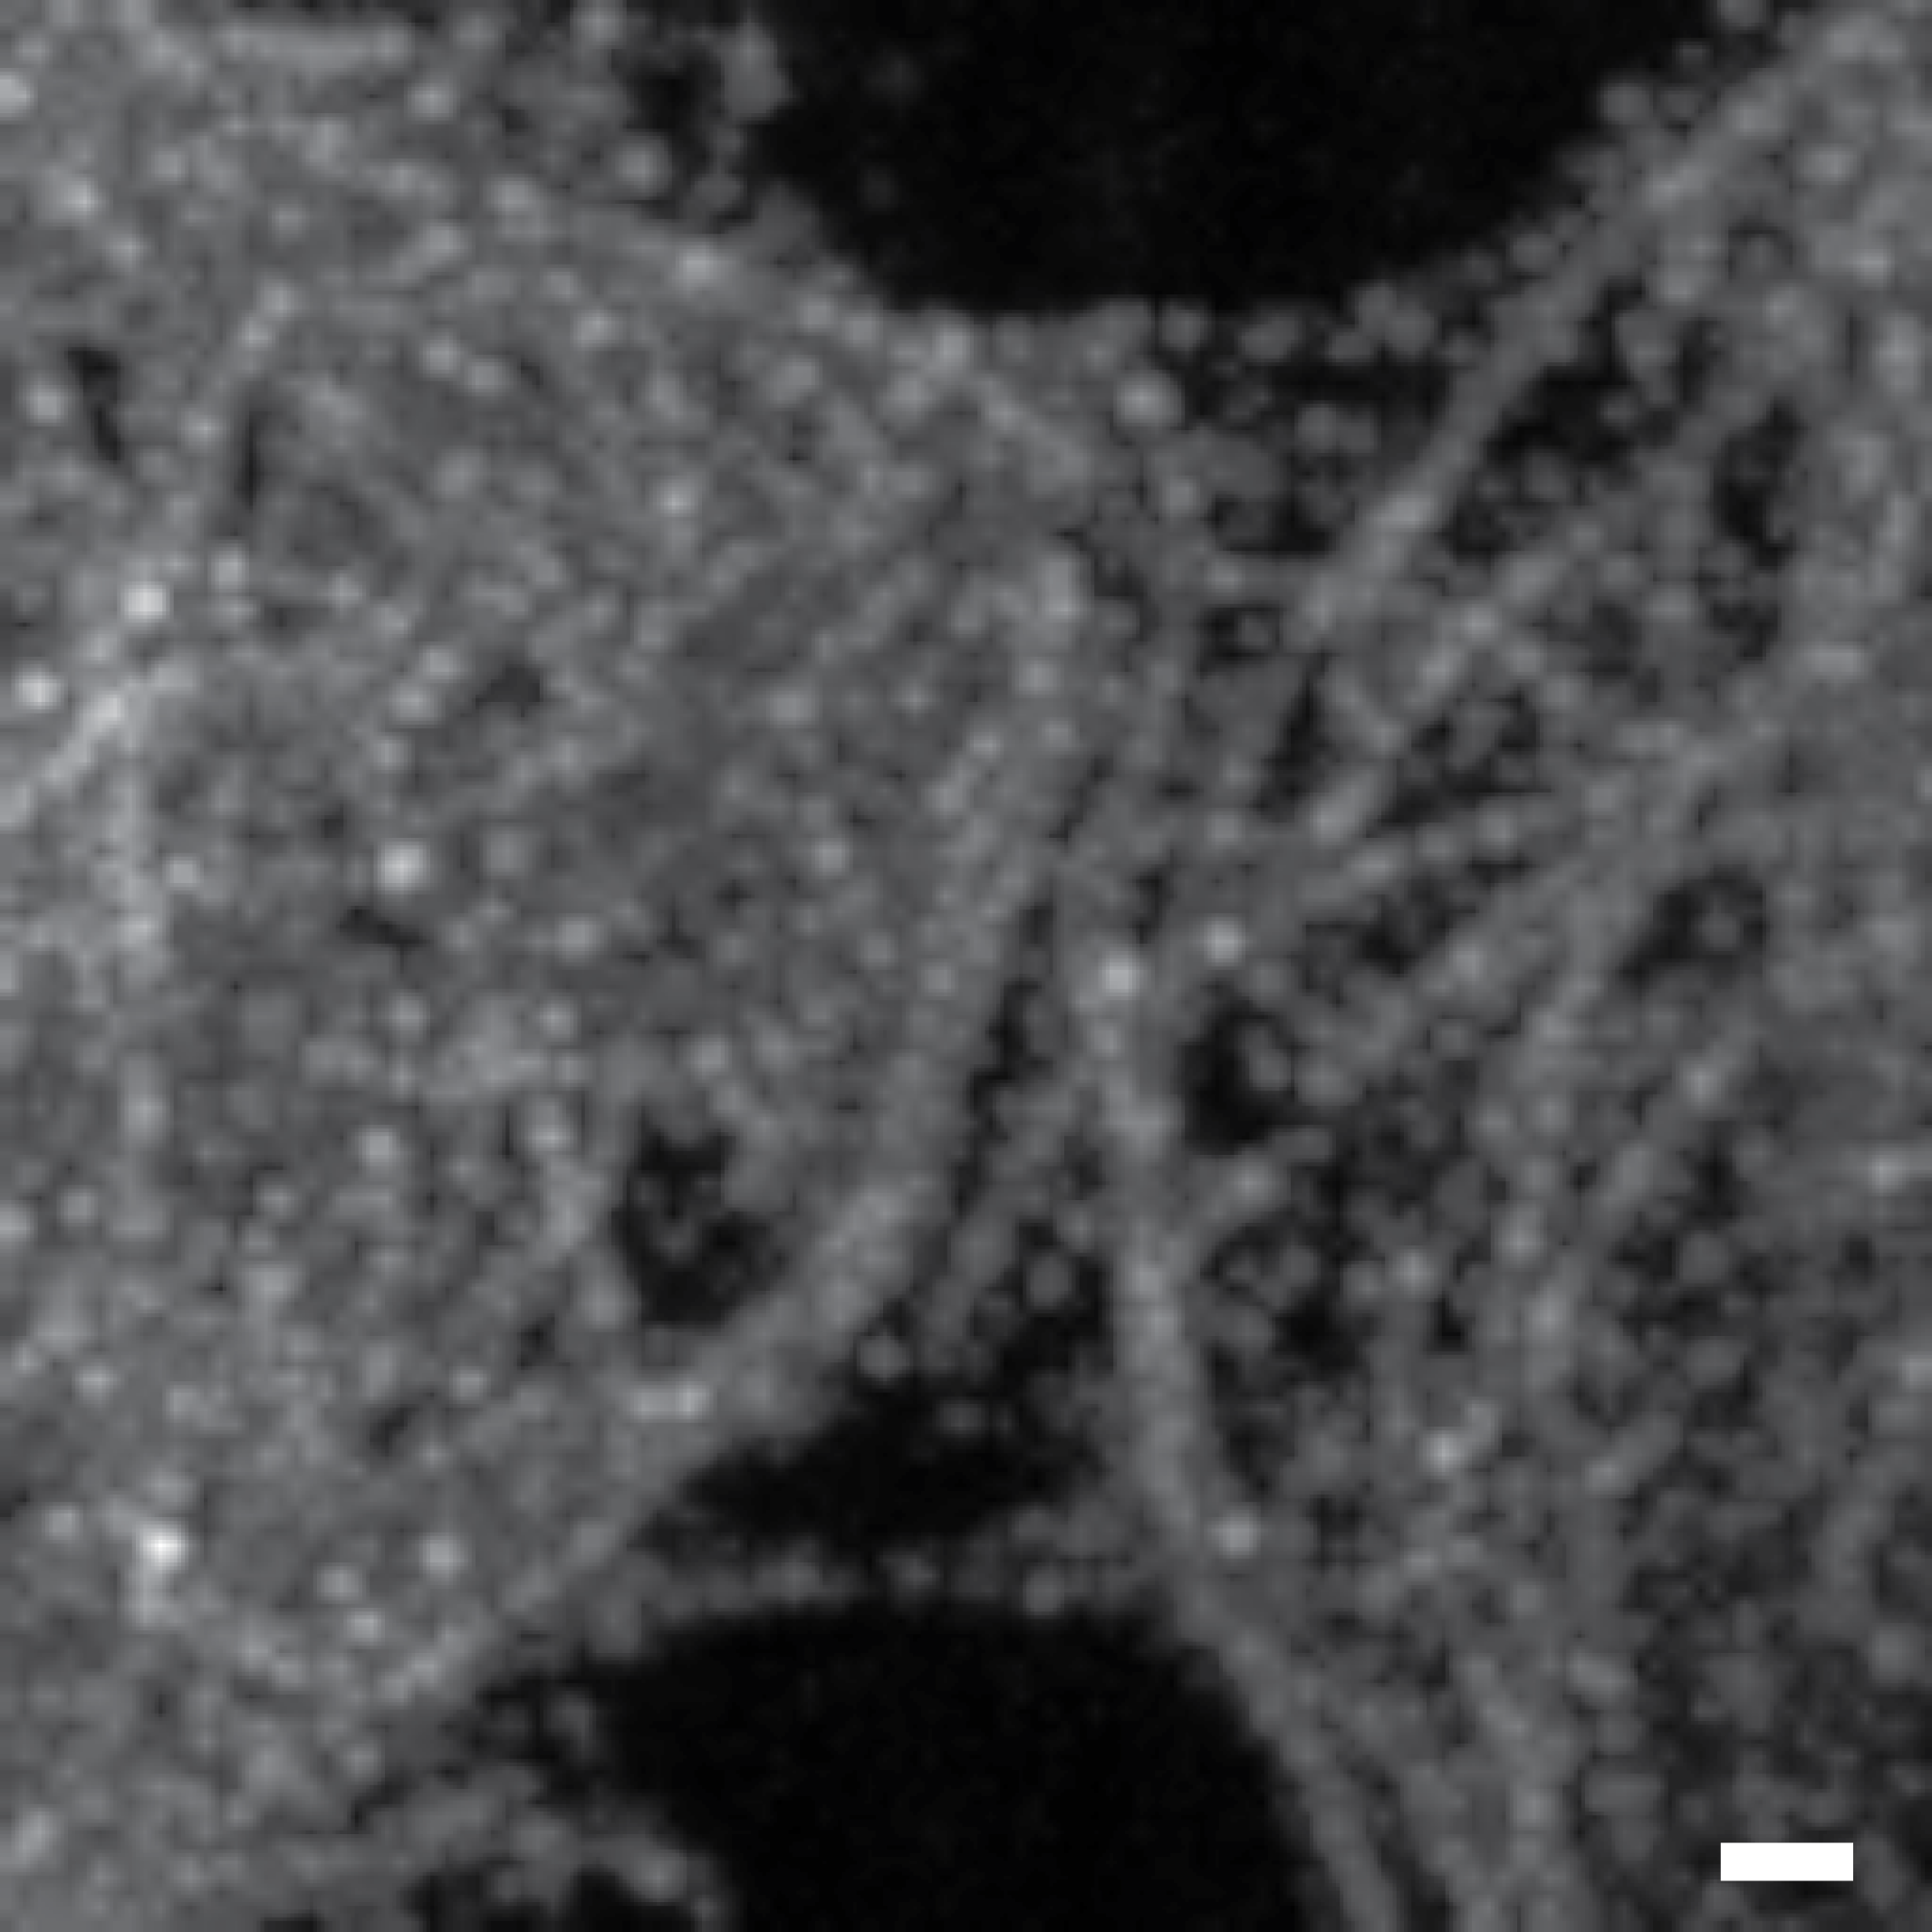
\includegraphics[width=0.45\textwidth]{figures/Bildmike_projection_scalebar}$\qquad$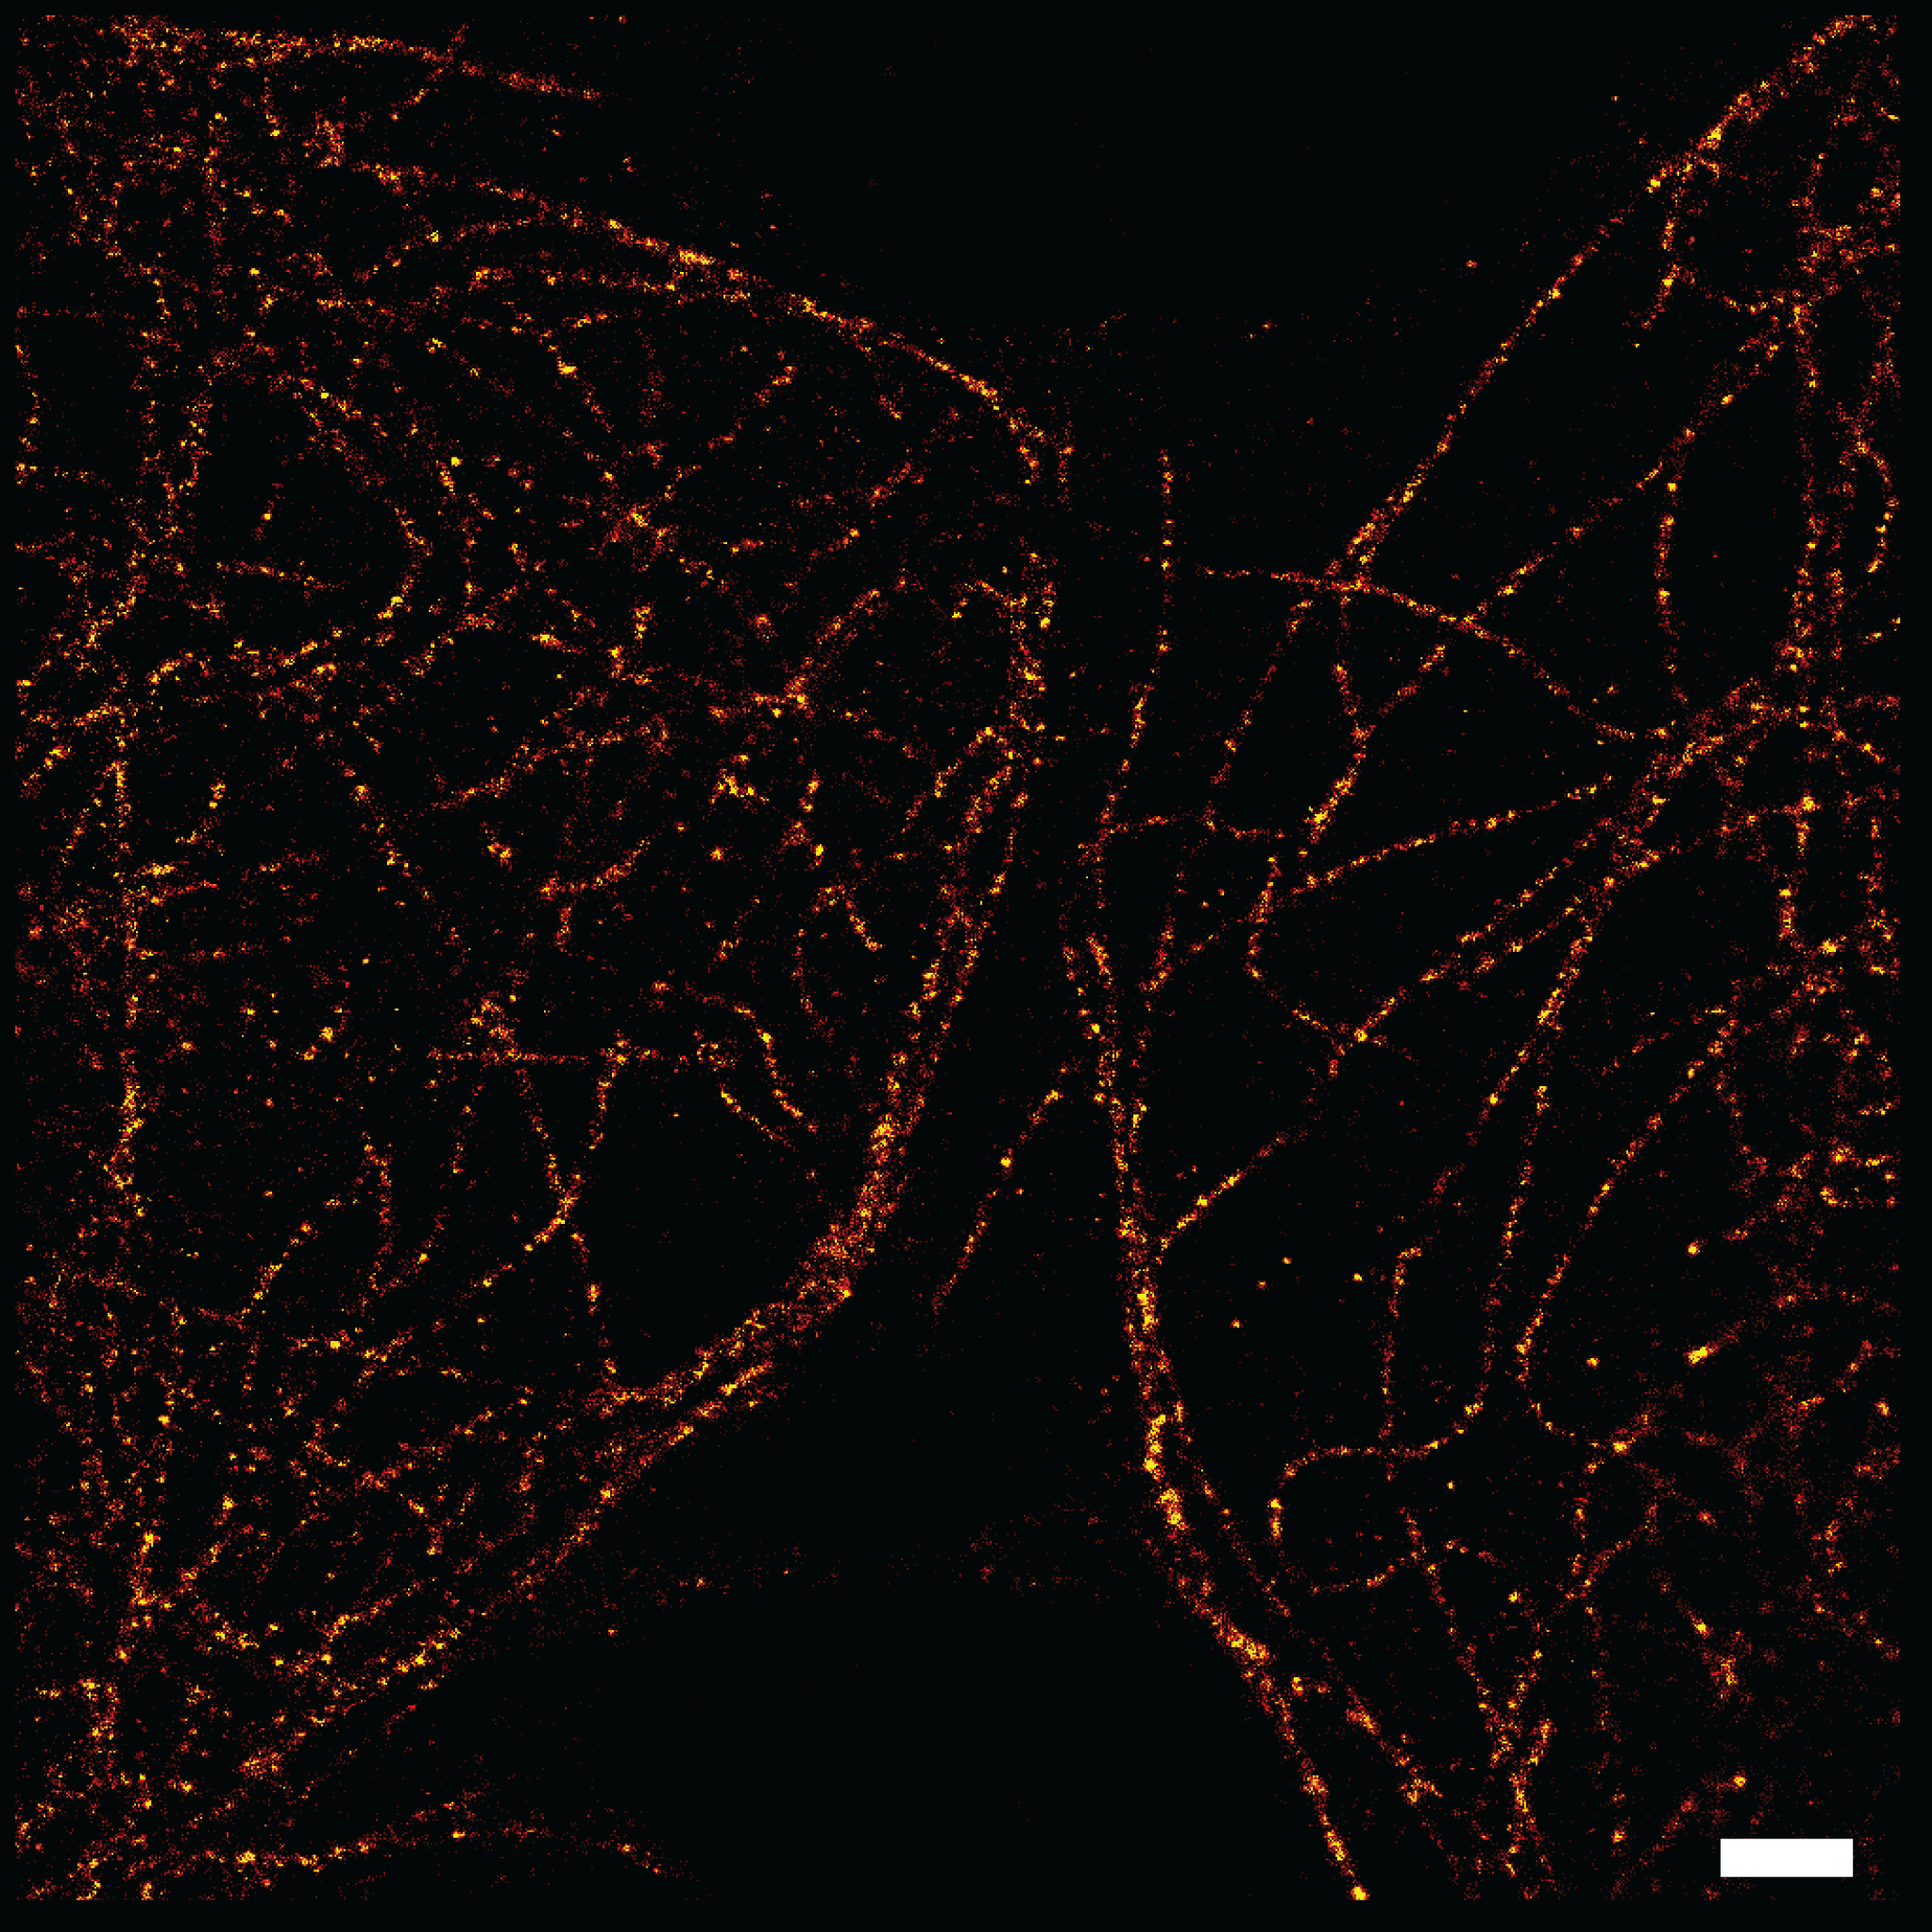
\includegraphics[width=0.45\textwidth]{figures/Bildmike_reconstruction_scalebar.png}
\par\end{centering}
\caption{Microtubuli, labeled with ATTO520 in HeLa-cells (data courtesy of Mike Heilemann).
Left: maximum projection of the raw data. Right: reconstructed high-resolution
image. Scalebar represents $1\mu m$}\label{fig:microtubuli}
\end{figure*}

\section{Related Work}\label{sec:related-work}

The classical reconstruction approach is based on direct fitting of
the PSF to every spot candidate. A model of the PSF with adjustable
parameters must be given. Usually, an isotropic Gaussian PSF like
(\ref{eq:gaussian-psf}) or an an\-iso\-tropic variant of it is sufficiently
accurate \citep{thompson_02_precise}, although alternative models may be required under certain cricumstances
\citep{stallinga_12_hermite-psf}. The free parameters of the
model are optimized by a non-linear fitting algorithm (e.g. the Levenberg-Marquart
method) in order to minimize the least-squares residual between the
fitted model and the intensities of a spot candidate. This method is the basis of the 
popular rapidSTORM software \citep{wolter_10_rapid-storm}, the ImageJ plugins Octane \citep{yu_11_octane}, PeakFit \citep{herbert_12_peakfit} and GraspJ (offering GPU acceleration, \cite{brede_12_graspj}), as well as the Localization Microscopy MicroManager plugin \citep{stuurman_12_plugin} and PYME (the Python localization microscopy environment, \cite{baddeley_12_pyme}).

An even simpler approach avoids iterative optimization by computing the centroid of 
each spot directly, either in terms of the intensity-weighted mean \citep{thompson_02_precise} or the 
fluoroBancroft method \citep{andersson_08_localization}. These methods were found to be only 
slightly less accurate then the least-squares fit when properly parametrized \citep{thompson_02_precise,hedde_09_localization-microscopy} and form the basis of fast reconstruction solutions such as the hardware-accelerated method of \citep{gruell_11_fpga-storm} and the QuickPALM ImageJ plugin \citep{henriques_10_quick-palm}.

Both fitting and direct methods have difficulties with the reconstruction of high density image sequences, because these images violate the basic model assumption that neighboring spots do not overlap. Greedy procedures for fitting overlapping spots where proposed by \citep{egner_07_nanoscopy}, who adapt H{\"o}gbom's classical CLEAN algorithm \citep{hoegbom_74_clean} to localization microscopy, the DAOSTORM algorithm from \citep{holden_11_daostorm}, an adaptation of DAOPHOT, a well-known algorithm from astronomy \citep{stetson_87_daophot}, and the multi-emitter fitting algorithm of \citep{huang_11_simultaneous}, who fit up to $N_{\max}$ overlapping PSFs simultaneously and select the most likely spot number by a statistical test. A more principled model for overlapping spots is provided by {\em compressed sensing} \citep{zhu_12_faster-storm}. Here, a PSF candidate is initialized at all pixels of a fine grid (e.g. having one-eighth the pixel size of the original image). The fit is then performed under a strong {\em sparsity prior} which ensures that only the center pixels of true spots get non-zero activation. While this method is more accurate than DAOSTORM, it is also very expensive (about a hundred times slower). Recently, substantial improvements of the sparse reconstruction approach have been achieved by more sophisticated modeling and optimization methods \citep{kim_13_localization-microscopy,min_13_localization-microscopy}. However, it is as yet unclear if the improvements over simple algorithms like SimpleSTORM warrant the added complexity.

Proper noise modeling is a critical ingredient for reliable distinction between true spots and noise artifacts. Many authors simply use a generic additive noise model and select spots whose intensity exceeds the background by a certain multiple of the background's noise standard deviation \citep{thompson_02_precise,gruell_11_fpga-storm}. Frequently, the image is preprocessed by averaging filters \citep{wolter_10_rapid-storm,huang_11_simultaneous}, Gaussian filters \citep{krizek_11_minimizing} or a wavelet transform \citep{izeddin_12_wavelet} before thresholding. However, non-uniform background intensity and intensity-dependent background noise make the choice of an appropriate threshold very difficult. Heuristic solutions to this problem lead to algorithms with many adjustable parameters that are very hard to use.

Moreover, it has been shown in \citep{abraham_09_localization-estimation} that a maximum likelihood fit based on a Poisson noise model outperforms the least-squares algorithm which implicitly assumes additive noise. A fast GPU-accelera\-ted version of this method is described in \citep{smith_10_fast}. However, the Poisson model cannot be applied directly to the observed image intensities because they deviate from the recorded photon counts due to the action of amplification. Amplified intensities are no longer Poisson distributed. The amplification can be inverted when gain factor and offset are known, but this requirement is apparently overlooked sometimes (e.g. \citep{andersson_08_localization,gruell_11_fpga-storm,brede_12_graspj}). A simple gain and offset estimation procedure using dedicated calibration images was proposed in \citep{lidke_05_photon-statistics}. A more convenient self-calibration algorithm was introduced in \citep{boulanger_10_patch-based}, who adaptively subdivide the given image sequence to determine regions of homogeneous intensity for gain estimation. This method is very similar in spirit to our approach in section \ref{sec:noise-normalization}, but their algorithm is considerably more complicated.

\section{Methods}
\subsection{\label{sec:matched-filters}Matched Filters}

It was shown by \citep{abraham_09_localization-estimation} that a maximum likelihood fit outperforms least-squares fitting when the noise follows a Poisson distribution. On the other hand, it is well-known that maximum likelihood and least-squares fitting are equivalent under additive Gaussian noise. Moreover, least-squares fitting can be replaced by {\em matched filtering} \citep{turin_60_matched-filters} when the mean background intensity is zero. Under these conditions, these algorithms are mathematically equivalent (as we show below), but filtering is much more efficient, in particular when the matched filter is a Gaussian PSF. This motivates our desire to work on {\em standardized images}, and robust standardization of the given image sequence is at the heart of the SimpleSTORM algorithm.
 
We briefly recall the relationship between matched filtering and least-squares fitting. Let the image $s(x,y)$ contain just a single spot with unknown scaling $\mu_0$ at an unknown location
$(x_{0},y_{0})$. We assume that the noise is additive Gaussian noise with mean zero
and variance $\sigma^{2}$, i.e. our image model is
\begin{eqnarray}
s(x,y) & = & f(x,y)+n(x,y)\label{eq:simple-signal-model}\\
 &  & f(x,y)=\mu_{0}\,\psf(x-x_{0},y-y_{0})\nonumber \\
 &  & n(x,y)\sim\mathcal{N}(0,\sigma^{2})\nonumber 
\end{eqnarray}
The least-squares algorithm determines the scaling $\mu_{m}$ and location $x_{m},y_{m}$ of a model $h(x,y)$ such that  the least-squares residual
\begin{multline}
\mu_{m}^{*},x_{m}^{*},y_{m}^{*}=\nonumber \\ 
\argmin_{\mu_{m},x_{m},y_{m}}\intRR\!\! \left(s(x,y)-\mu_{m}h(x-x_{m},y-y_{m})\right)^{2}\,d\vec{x}
\end{multline}
is minimized. After expanding the integrand, this is equal to
\begin{multline}
\argmin_{\mu_{m},x_{m},y_{m}}\intRR\!\! s(x,y)^{2}\,d\vec{x}+\mu_{m}^{2}\intRR\!\! h(x-x_{m},y-y_{m})^{2}\,d\vec{x}\nonumber \\
\hfill -2\mu_{m}\intRR\!\! f(x,y)h(x-x_{m},y-y_{m})\, d\vec{x}\quad\, \\
-2\mu_{m}\intRR\!\! n(x,y)h(x-x_{m},y-y_{m})\, d\vec{x}
\end{multline}
The first integral is a constant (since the signal is fixed), the
last one has zero expected value (since the noise is uncorrelated),
and both terms can be dropped from the optimization. After reversing the
sign, we obtain the equivalent optimization problem
\begin{multline}
\argmax_{\mu_{m},x_{m},y_{m}}2\mu_{m}\intRR\!\! f(x,y)h(x-x_{m},y-y_{m})\, d\vec{x}\nonumber \\
-\mu_{m}^{2}\intRR\!\! h(x-x_{m},y-y_{m})^{2}\,d\vec{x}
\end{multline}
Setting the derivative w.r.t. $\mu_{m}$ to zero gives an analytic solution for $\mu^*_m$
\[
\mu^*_{m}=\frac{\intRR f(x,y)h(x-x_{m},y-y_{m})\, d\vec{x}}{\intRR h(x-x_{m},y-y_{m})^{2}\,d\vec{x}}
\]
resulting in a reduced optimization problem for the location
\[
x_{m}^{*},y_{m}^{*}=\argmax_{x_{m},y_{m}}\frac{\left(\intRR f(x,y)h(x-x_{m},y-y_{m})\, d\vec{x}\right)^{2}}{\intRR h(x-x_{m},y-y_{m})^{2}\,d\vec{x}}
\]
The numerator is the squared correlation function between $ f(x,y)$ and $h(x-x_{m},y-y_{m})$. Expanding it in terms of the  Cauchy-Schwarz inequality yields
\begin{eqnarray}
\lefteqn{\frac{\left(\intRR f(x,y)h(x-x_{m},y-y_{m})\, d\vec{x}\right)^{2}}{\intRR h(x-x_{m},y-y_{m})^{2}\,d\vec{x}}}\nonumber \\
&\qquad\qquad&\le\frac{\intRR f(x,y)^{2}\, d\vec{x}\cdot\intRR h(x-x_{m},y-y_{m})^{2}\, d\vec{x}}{\intRR h(x-x_{m},y-y_{m})^{2}\,d\vec{x}}\nonumber \\
&&=\intRR\!\! f(x,y)^{2}\, d\vec{x}=\mathrm{const.}\nonumber
\end{eqnarray}
and equality (i.e. the maximum possible value) is only achievable when $h(x-x_{m},y-y_{m})=\kappa\, f(x,y)$.
The maximum is thus obtained for $x_{m}^{*}=x_{0}$ and $y_{m}^{*}=y_{0}$ as desired. Since $\kappa$ can be chosen arbitrarily, $h(x,y)$ can be defined as a \emph{matched filter}
\[
h(x,y)=\psf(x,y)
\]
The optimal estimate of the spot location is therefore the point where
the convolution
\begin{equation}
%x_{m}^{*},y_{m}^{*}=\argmax_{x,y}g(x,y)=\psf(x,y)\star s(x,y)
g(x,y)=\psf(-x,-y)\star s(x,y)
\end{equation}
assumes its maximum (recall that correlation is equivalent to convolution with the mirrored kernel). This point can be conveniently determined by
spline interpolation of $g$, see section \ref{sec:spot-localization}.


To use matched filters in localization microscopy, the following requirements
must be met:
\begin{enumerate}
\item The PSF must be known. We address PSF estimation in section \ref{sec:psf-estimation}.
\item The PSF should be uniform throughout the image. This condition may
not be fulfilled when some spots are out of focus. However, this is
not a major problem in practice, because the filter $h$ degrades
gracefully: Although no longer the best possible filter, it still
performs reasonably as long as the PSF is not too far off. 
\item Each image should contain only one spot. This is clearly violated
in practice and in fact undesirable. But this is no problem as long as the spot density is not too high. Since the PSF
decreases quickly, the filter response at point $(x,y)$ is not influenced
by spots that are sufficiently far away. The detector suffers only
a minor degradation at overlapping spots
whose distance remains larger than the PSFs full width at half
maximum (FWHM). The spot density can easily be controlled by the experimental
setup.
\item The image's background intensity must be zero. We use a standard background
subtraction procedure as described in section \ref{sec:background-subtraction}.
\item The noise must be additive Gaussian. This is the most serious obstacle,
because the noise variance is actually a function of the intensity and therefore
not additive. To rescue the matched filter approach, we transform
the original image intensities so that the noise is approximately
turned into additive Gaussian noise. Our \emph{noise normalization}
procedure is described in section \ref{sec:noise-normalization}.
\end{enumerate}

\subsection{\label{sec:noise-normalization}Noise Normalization}

Matched filtering is only optimal when the noise is additive and Gaussian
distributed. However, localization microscopy is based on a photon
counting process, which instead follows a Poisson distribution with
intensity-dependent variance. The probability of observing $k$ photons
in pixel $(x,y)$ is given by
\[
p\left(k\right)=\frac{\lambda^{k}}{k!}e^{-\lambda}
\]
where $\lambda=\lambda(x,y)$ is the expected count, i.e. true intensity (we dropped the dependency on $(x,y)$ to improve readability). Moreover,
these counts are not observed directly but are subjected to several
amplification stages and discretized into a finite set of gray levels.
If we assume linear amplification characteristics and neglect discretization
effects%
\footnote{This is possible because the discretization noise is typically much smaller
than the noise from other sources.%
}, the observed image gray levels $k'$ depend on $k$ according to
the linear function 
\begin{equation}
k'=a\, k+b\label{eq:linear-gain-model}
\end{equation}
where $a$ denotes the total gain factor and $b$ the
dark signal (offset). The noise in $k'$ is no longer Poisson distributed.
One can easily see this by recalling that both the mean and variance
of a Poisson distribution are equal to $\lambda$. In contrast, mean
and variance of $k'$ are
\begin{eqnarray*}
E\left[k'\right] & = & a\, E\left[k\right]+b=a\,\lambda+b\\
\var\left[k'\right] & = & a^{2}\, \var\left[k\right]=a^{2}\lambda
\end{eqnarray*}
and these quantities are in general different. Consequently, it is \emph{incorrect}
to apply algorithms which rest
on the assumption of Poisson or Gaussian noise (like matched filtering) directly to the observed
image $k'(x,y)$. Fortunately,
there is an easy way out: the \emph{Anscombe transform} \citep{anscombe_48_noise-normalization}
\[
q(x,y)=2\sqrt{k(x,y)+\frac{3}{8}}
\]
turns a Poisson distributed signal $k(x,y)$ into an approximately
Gaussian distributed one $q(x,y)$ with unit variance, regardless
of the value of $k$ (as long as $k\ge4$). However, in order to apply
the Anscombe transform, we need to know the coefficients $a$ and
$b$ that map the observed gray values $k'$ back into the Poisson
distributed counts $k$:
\begin{equation}
q(x,y)=2\sqrt{\frac{k'(x,y)-b}{a}+\frac{3}{8}}\label{eq:anscombe-transform}
\end{equation}
Determining $a$ and $b$ turns out to be tricky. The standard
solution is to record dedicated calibration images where the mean
and variance of $k'$ can be computed easily \citep{lidke_05_photon-statistics}. Then, a linear regression
through a set of pairs $\left(E[k'],\, \var[k']\right)$ with different
$k'$ directly provides the desired coefficients. However, this approach
is inconvenient when the camera is mounted on a microscope.
Therefore, we seek to determine these coefficients from the raw localization images themselves by self-calibration. 

Among a large number of ideas we tried, the following turned out to
be the most stable. Consider a pixel $(x,y)$ whose true intensity is
constant over time, i.e. the pixel shows background or a bead,
but no blinking molecule. Then we can easily compute its average intensity
and variance over time and obtain a point for the linear regression.
The difficulty is that we do not know which pixels have this property.
The following consideration shows a way to identify them: Whenever
the true intensity is not constant, the apparent variance is larger
than it would otherwise be, because
\[
\var\left[f(t)+n(t)\right]=\var\left[f(t)\right]+\var\left[n(t)\right]
\]
where $f(t)$ is a time-dependent signal and $n(t)$ denotes noise
which is uncorrelated with the temporal behavior of $f$. When $f(t)=\mathrm{const.}$, its variance is zero, resulting in
the minimal possible value of $\var\left[f(t)+n(t)\right]$. Otherwise,
the total variance increases. This leads to the following algorithm
\begin{enumerate}
\item Select $n$ image locations at random.
\item Compute mean and variance of the corresponding pixels over the first
$T$ frames of the sequence ($T=200$ works well in practice, but
the value can be adjusted). Create the scatter plot of the resulting
mean/variance pairs.
\item Use the RANSAC algorithm \citep{fischler_81_ransac} to compute the lower leaning line of the
scatter plot: Repeat $k=10000$ times:

\begin{enumerate}
\item Select two points at random and compute the line through these points.
\item Determine the number of inliers of this line, i.e. the number of points
whose distance from the line is at most a twentieth of the range between the minimal and the maximal value.
\item Keep the line with the maximum number of inliers as the best estimate
of the lower leaning line.
\end{enumerate}
\item The coefficients $a$ and $b$ now correspond to the slope and intercept
of the lower leaning line, because this line contains precisely the
points whose intensity was constant over time. All points not near
the lower leaning line are ``contaminated'' by intensity variations
and therefore ignored. 
\end{enumerate}
\begin{figure}
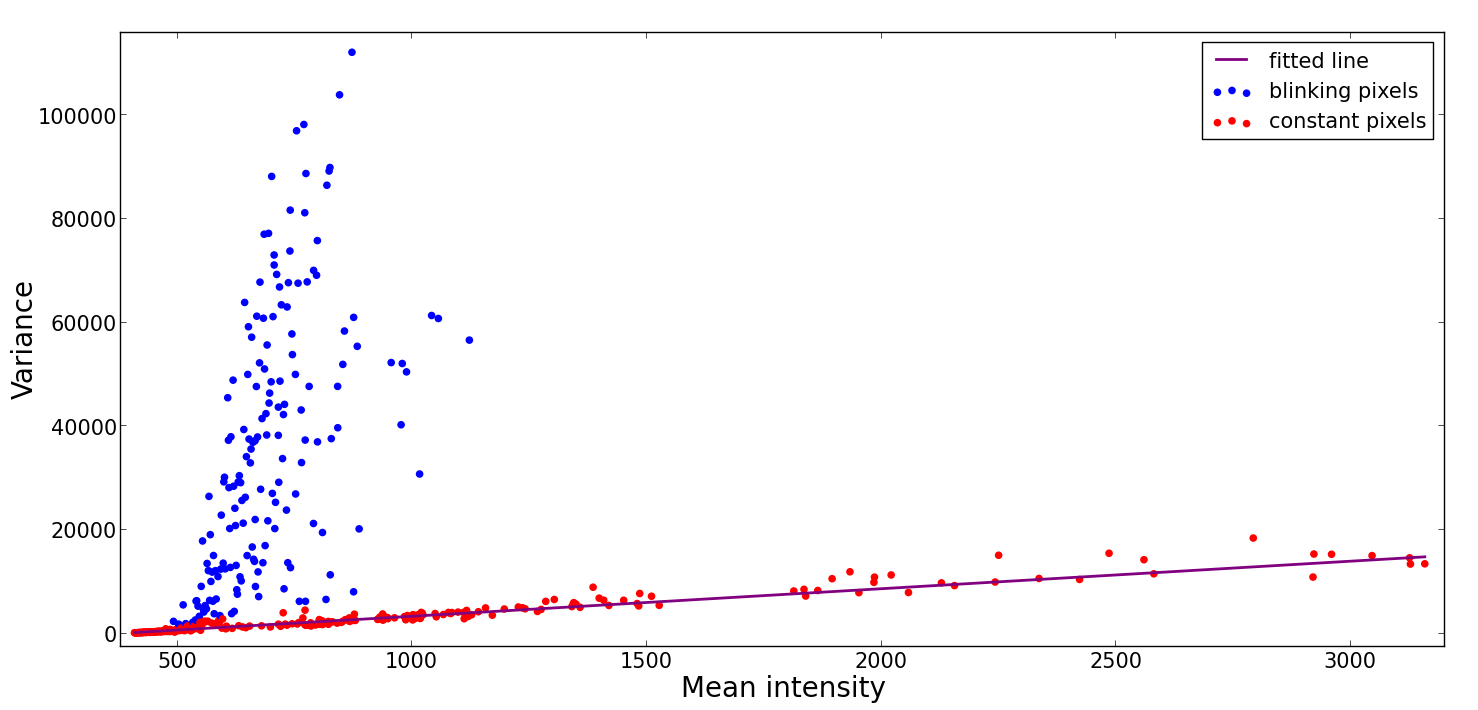
\includegraphics[width=1\columnwidth]{figures/lower-leaning-line}
\caption{\label{fig:lower-leaning-line}RANSAC-fitting of a lower leaning line
to a scatter plot showing variance vs. mean intensity for randomly
selected pixels. Slope and intercept of this line determine the correction
coefficients in equation (\ref{eq:anscombe-transform}).}
\end{figure}
Figure \ref{fig:lower-leaning-line} shows an example of the fit
according to this algorithm. It can be seen that it does indeed detect
the lower leaning line of the scatter plot, which corresponds to the
pixels with constant intensity.

Occasionally, the range of intensities on the lower leaning line is rather small (e.g. when no beads are present), resulting in noisy gain estimates. This can be fixed by iterative post-optimization: We use the estimated parameters to transform the 
data according to (\ref{eq:anscombe-transform}) and compute an intensity histogram for each of the first 200 frames. These histograms contain mixture distributions with one mixture component for the background and one for the rest. We fit a Gaussian to the background mixture component in each histogram and compute the average variance of these Gaussians. When this value is not within $5\%$ of unity, the gain factor is multiplied with the measured variance and the procedure repeated. This algorithms leads to stable gain estimates within a few iterations.

\subsection{\label{sec:background-subtraction}Background Subtraction}

Once the noise model is known, we transform the observed images $k_{t}'(x,y)$
into noise-normalized ones $q_{t}(x,y)$ (where $t$ indicates time) according to section \ref{sec:noise-normalization}. The next step is the estimation
of the background intensity. It is based on the standard assumption
that the background varies much slower then the actual
signal both spatially and over time. We split the dataset into non-overlapping
blocks of size $\rho^{2}\times\tau$, where $\rho$ is the block size
in the two spatial directions, and $\text{\ensuremath{\tau}}$ is
the block size along the time direction. Default values of $\rho=30$
and $\tau=20$ work well in all our experiments. If necessary, the
user can adjust these settings. This is easy because he or she can determine
how fast the background varies by simple visual inspection of the
data. 

In each block, the median of the gray values $s$ is computed. The
median is preferable to the mean because it is more stable when the
block contains non-background pixels (blinking spots and beads): These
pixels lead to a significant upward bias in the mean, whereas the
median increases only marginally. The median values are placed on
the grid points defined by the centers of the blocks, and interpolated to
the original image resolution (both in spatial and time direction)
using a Catmull-Rom spline which ensures smooth (i.e. differentiable)
interpolation and thus avoids blocking artifacts in the background
estimate $\beta_{t}(x,y)$. After subtracting $\beta_{t}$ from the
noise normalized signal $q_{t}$, we obtain the signal $s_{t}$ which
has unit variance in all pixels and zero mean in the background:
\begin{equation}
s_{t}(x,y)=q_{t}(x,y)-\beta_{t}(x,y)\label{eq:background-subtraction}
\end{equation}
We call the resulting image $s_{t}$ the {\em standardized} image because it 
now conforms to the requirements of the matched
filter method. Figure \ref{fig:background-subtraction}
shows examples.
\begin{figure*}

\includegraphics[width=0.3\textwidth]{figures/Tubulin2OrigFrame50}$\qquad$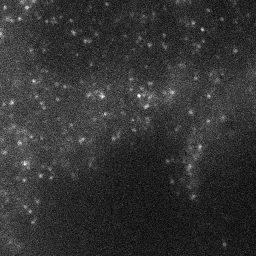
\includegraphics[width=0.3\textwidth]{figures/dcframe4.png}$\qquad$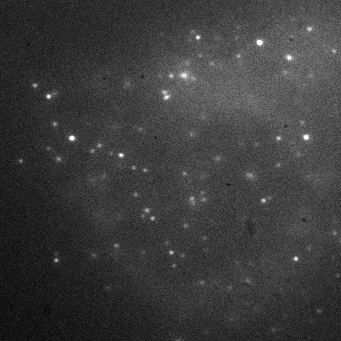
\includegraphics[width=0.3\textwidth]{figures/lunet_raw_frame2547_rotated4.png}\\[6pt]
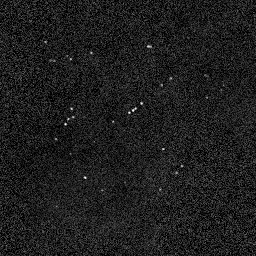
\includegraphics[width=0.3\textwidth]{figures/Tubulin2normalprocessFrame50}$\qquad$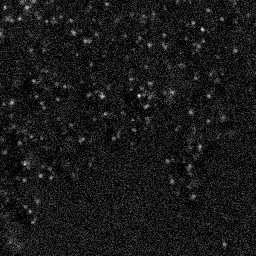
\includegraphics[width=0.3\textwidth]{figures/dcframe4_bgsubtracted.png}$\qquad$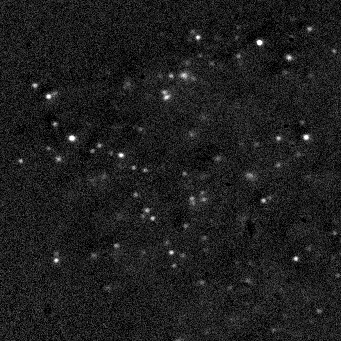
\includegraphics[width=0.3\textwidth]{figures/lunet_processed_rotated4.png}

\caption{\label{fig:background-subtraction}Top: original images (from left: frame 50
of the artificial Tubulin2 dataset, actin conjugated to mEos2, and tubulin labeld with Cy5, see section \ref{sec:results} for details on the data). Bottom: the same frames after standardization.}
\end{figure*}


\subsection{\label{sec:psf-estimation}Estimation of the PSF}

In order to apply the matched filter method, an accurate estimate of the PSF is required. We investigated two approaches to PSF estimation, a non-parametric and a parametric one. In both cases, the PSF is estimated by averaging over many spots {\em after} image standardization. The non-parametric method determines the PSF in the form of an optimal \emph{Wiener filter} which is based on the \emph{magnitude spectrum}
of the signal. Let
\[
S_{t}=\mathcal{F}[s_{t}]
\]
the Fourier transform of standardized frame $s_{t}$. Then the average power spectrum over
T frames is
\[
P=\frac{1}{T}\sum_{t=1}^{T}\left|S_{t}\right|^{2}
\]
where $\left|S_{t}\right|$ is the point-wise magnitude of the complex
frequency response. The Wiener filter is then defined as
\[
W=\left(\frac{P-P_{\mathrm{noise}}}{P}\right)_{+}
\]
where $P_{\mathrm{noise}}$ is the expected power spectrum of the noise and $\left(.\right)_{+}=\max\left(0,.\right)$
is the hinge function that truncates negative values at zero (negative
values can occur because we estimate $W$ from a finite sample). Since the noise (after standardization) is additive Gaussian noise with zero mean and unit variance,
its expected power spectrum is simply $P_{\mathrm{noise}}=1$. The matched filter
can now be computed by multiplication of each frame's Fourier transform
with the Wiener filter, followed by inverse Fourier transform
\[
\hat{s}_{t}=\mathcal{F}^{-1}[S_{t}\cdot W]
\]
In contrast, the parametric method assumes that the PSF is shaped
like a Gaussian, which is a very good approximation for typical microscopes.
Under this assumption, the self-calibration only needs to determine
a single parameter, the PSF scale $\sigma_{\psf}$. Clearly, the variance of a single
parameter estimate is much smaller than the variance of an entire
non-parametric PSF estimate when the same number of samples are used. The Gaussian
model is therefore preferable when it conforms to the actual PSF shape,
whereas the Wiener filter should be applied otherwise. Due to image standardization, our estimate $\sigma_{\psf}$ is related to the PSF size $\sigma^*_{\psf}$ of the raw data by the relation $\sigma_{\psf}=\sqrt{2}\,\sigma^*_{\psf}$.

The Gaussian fit can be performed both in the spatial and in the Fourier
domain. The Fourier domain approach starts in the same way as in the
non-parametric case, i.e. we compute the average power spectrum of
the noise-normalized signal. To simplify subsequent computations,
we cut out sufficiently large {\em square} ROIs from the original
frames and compute their average power spectrum $P'$. Now, instead
of using the power spectrum directly to define a Wiener filter, we
compute the average magnitude spectrum $\sqrt{P'}$ and use it to
fit a Gaussian function. Since the Fourier transform of a Gaussian
PSF and the corresponding magnitude spectrum are again rotationally
symmetric Gaussian functions, the model is 
\begin{equation}
g(r | w_1, w_2, w_3) = w_{1}\,\exp\left(-\frac{r^{2}}{2w_{2}^{2}}\right)+w_{3}\label{eq:gaussian-psf}
\end{equation}
where $r=\sqrt{u^{2}+v^{2}}$ is the distance of the point from the
origin. The parameters $w_{i}$ are chosen by means of non-linear
least-squares optimization (using the Levenberg-Marquardt algorithm) such that
the squared difference between the model and the power spectrum is
minimized
\[
w_{1},w_{2},w_{3}=\argmin_{w_{i}}\sum_{u,v}\left[g(r | w_1, w_2, w_3)-\sqrt{P'(r)}\right]^{2}
\]
Parameters $w_{1}$ and $w_{3}$ account for the signal and noise
intensities respectively, whereas the desired PSF scale in the spatial
domain can be obtained from the parameter $w_{2}$ by the simple relation
\[
\sigma_{\psf}=\frac{W}{2\pi w_{2}}
\]
where $W$ is the width of the ROI used to compute the magnitude spectrum
(recall that we select squared ROIs to simplify matters). The fit
in the spatial domain is performed similarly, but the simple averaging
via the average power spectrum is not possible here. Instead, we fit
the PSF independently to a number of easy-to-detect spots, and then
define $\sigma_{\psf}$ as the median of the parameter $w_2$ of the individual estimates.
(Thus, we also use the standard fitting algorithm of \citep{thompson_02_precise}, but only to estimate $\sigma_{\psf}$.)

Finally, the result of matched filtering is 
\[
\hat{g}_{t}=s_{t}\star\mathrm{gauss}_{\sigma_{\psf}}
\]
where $\star$ denotes convolution. Experimental results are reported in section \ref{sec:validation}

\subsection{Spot Detection}\label{sec:spot-detection}

Spot detection is performed in each frame after image standardization. Since the background now contains only Gaussian additive noise with zero mean and unit variance,
a standard statistical test can be used to detect pixels whose intensity
is unlikely to be background. For a given $p$-value, corresponding
to the probability of false positives, the intensity threshold is
\begin{equation}
t\ge\sqrt{2}\,\erfi(2p-1)\label{eq:detection-threshold}
\end{equation}
where $\erfi(.)$ is the inverse error function. That is, a
normalized pixel with intensity at least $t$ has a probability of
at most $p$ to represent background. For example, $p$-values of
1\% and 0.1\% correspond to thresholds 2.3 and 3.1 and indicate that
one gets one false positive on average per 10x10 and 30x30 window
respectively. Note that these thresholds are independent of the image
content. In contrast to many existing algorithms, there is no need for manual threshold adjustment or complicated threshold
selection heuristics in SimpleSTORM.

The false positive rate can be further reduced 
by noticing that true spots always cover several pixels, whereas the noise in neighboring pixels is uncorrelated.
Therefore, the probability that multiple adjacent pixels are above threshold
\emph{simultaneously} is low for background pixels, but high for true spots. In practice, we accept
a spot if at least three connected pixels exceed the threshold for
the chosen $p$-value. The probability of false positives in this
setting can be approximated by a binomial distribution with parameter
$p$. For example, for $p=1\%$, the probability that three or more
background pixels are above threshold in a given 3x3 window is below
$0.01\%$, for $p=0.1\%$ the resulting probability is $\approx\!10^{-5}\%$. 
The result of this step is a set of spot masks, i.e. connected regions
above threshold that contain at least three pixels.


\subsection{\label{sec:spot-localization}Spot Localization}

In order to perform spot localization, we first subject the normalized
image to the matched filter described in section \ref{sec:matched-filters},
i.e. we filter with a Gaussian whose size $\sigma_{\psf}$ has
been determined according to section \ref{sec:psf-estimation}. We
don't apply this filter before spot \emph{detection} because this
would introduce complicated correlation between the noise of neighboring
pixels, making the distinction between signal and noise more difficult. 

The theory of matched filtering suggests that each local maximum of
the filtered image corresponds to a location of best match between
the data and the spot model. This location needs to be determined
to subpixel accuracy, and a residual error of 1/5 to 1/10 of a pixel is typically
achievable. The simplest possibility to do so is via cubic spline
interpolation of the filtered image to the desired resolution. The
upsampling ratio can be chosen by the user and is typically between
8 and 16. To save time, the interpolation is only performed in sufficiently
large rectangles around each spot mask (i.e. the bounding rectangle
plus four pixels in every direction). Each local maximum of the interpolated
image which is covered by one of the spot masks is returned as a detected
spot. 

Important spot properties such as signal-to-noise ratio and anisotropy
can be readily obtained from the properties of the interpolated image.
Let $g$ be the intensity of the interpolated image at the local maximum
position, and $g_{xx}$, $g_{xy}$, $g_{yy}$ the corresponding second
derivatives (these derivatives can be easily computed analytically
from the spline representation). Then the following relations can be derived from basic properties of Gaussian functions. Since the noise has unit variance before matched filtering, the (unfiltered) signal-to-noise ratio is simply
given by  
\[
\snr=2g
\]
(the factor of 2 accounts for the smoothing effect of the matched
filter). The standard deviation of the 2D localization error $\Delta \vec{x}$ after matched filtering, defined in units of the pixel spacing, is then
\begin{equation}
\mathrm{StdDev}[\Delta \vec{x}]=\frac{1}{\sqrt{\pi}\,g}\label{eq:spot-std-dev}
\end{equation}
This is of the expected form, because $g$ is proportional to $\sqrt{N}$ (the square root of the photon count) due to the action of the Anscombe transform.

The maximum and minimum radius of a potentially anisotropic spot can be computed from the eigenvalues
of the second derivative matrix
\[
\kappa_{1,2}=\frac{1}{2}\left(g_{xx}+g_{yy}\pm\sqrt{g_{xx}^{2}+g_{yy}^{2}+4\, g_{xy}^{2}-2\, g_{xx}g_{yy}}\right)
\]
by the expressions
\begin{eqnarray*}
s_{\max} & = & \sqrt{-g/\kappa_{1}-\sigma_{\mathrm{filter}}^{2}}\\
s_{\min} & = & \sqrt{-g/\kappa_{2}-\sigma_{\mathrm{filter}}^{2}}
\end{eqnarray*}
(with $\sigma_{\mathrm{filter}}=\sigma_{\psf}$ for matched filtering) and their ratio gives the spot anisotropy

\[
\mbox{AI}=\frac{s_{\max}}{s_{\min}}
\]
Spot radii and anisotropy can serve as additional selection criteria
to remove undesired anisotropic spots, or as a means to determine
spot depth in 3D localization microscopy with cylindrical lenses.

It should be noted that each spot mask can contain multiple local
maxima. This is desirable because it allows us to detect overlapping
spots, provided that the overlap is not too big. Specifically, when we skip the filtering step altogether and detect maxima directly in the interpolated standardized images, overlapping
spots of equal intensity remain separable (i.e. give rise to distinct
maxima) when the distance of their centers exceeds $2\,\sigma_{\psf}$.
The localization error $\Delta \bm{x}'$ then becomes
\[
\mathrm{StdDev}[\Delta \vec{x}']=\frac{\pi\,\sigma^2_{\psf}}{\sqrt{3}\,g'}
\]
where $g'$ is the intensity at the location of the maximum and $\sigma_{\psf}$ is taken in units of the pixel spacing.
This possibility is an advantage of our method over reconstruction
algorithms that explicitly fit the PSF to the image data: The fitting
approach only works reliably when the spots do not overlap significantly,
i.e. when the spot distance is about twice as big.


\section{Results}\label{sec:results}
\subsection{Validation Datasets}\label{sec:validation}
Validation data should be both realistic and accompanied with ground truth. A good compromise between these conflicting goals is achieved by the simulated image sequences that have been designed with great care for the ISBI Single-Molecule Localization Microscopy Challenge 2013 and can be downloaded freely\footnote{\url{http://bigwww.epfl.ch/smlm/datasets/index.html}}. The ground truth is available for four ``training'' data\-sets,and we used these for most of our quantitative experiments. Six additional datasets with undisclosed ground truth were used in the contest, where SimpleSTORM also performed well. Since the organizers did not yet publish the results officially, we compiled the ranking charts in figure \ref{scatterplot_challenge} from the material handed out at the competition workshop. The charts place each participant according to the average ranking in two performance metrics (Jaccard index and RMSE, see below) in the ``high spot density'' and ``low spot density'' data categories.
\begin{figure}
\begin{centering}
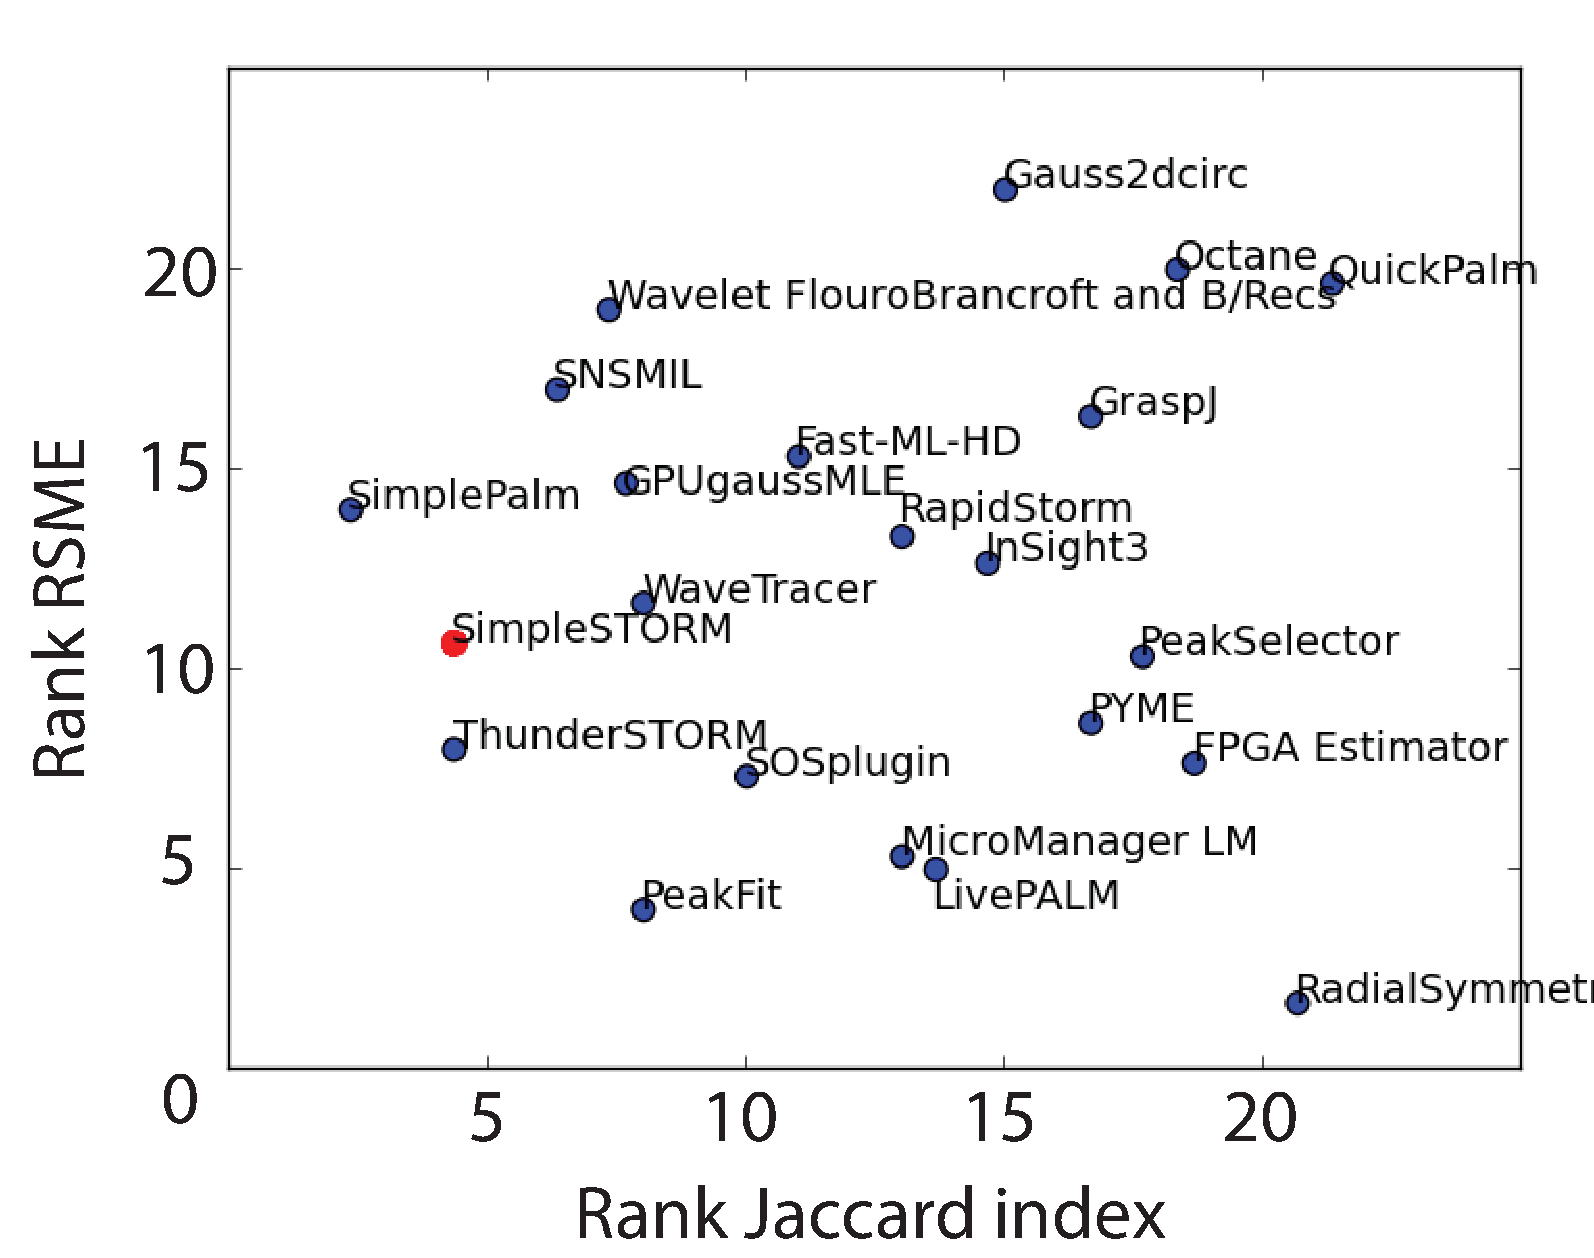
\includegraphics[width = 0.4\textwidth]{figures/low_Density_scatter.pdf}\hspace{1cm}%
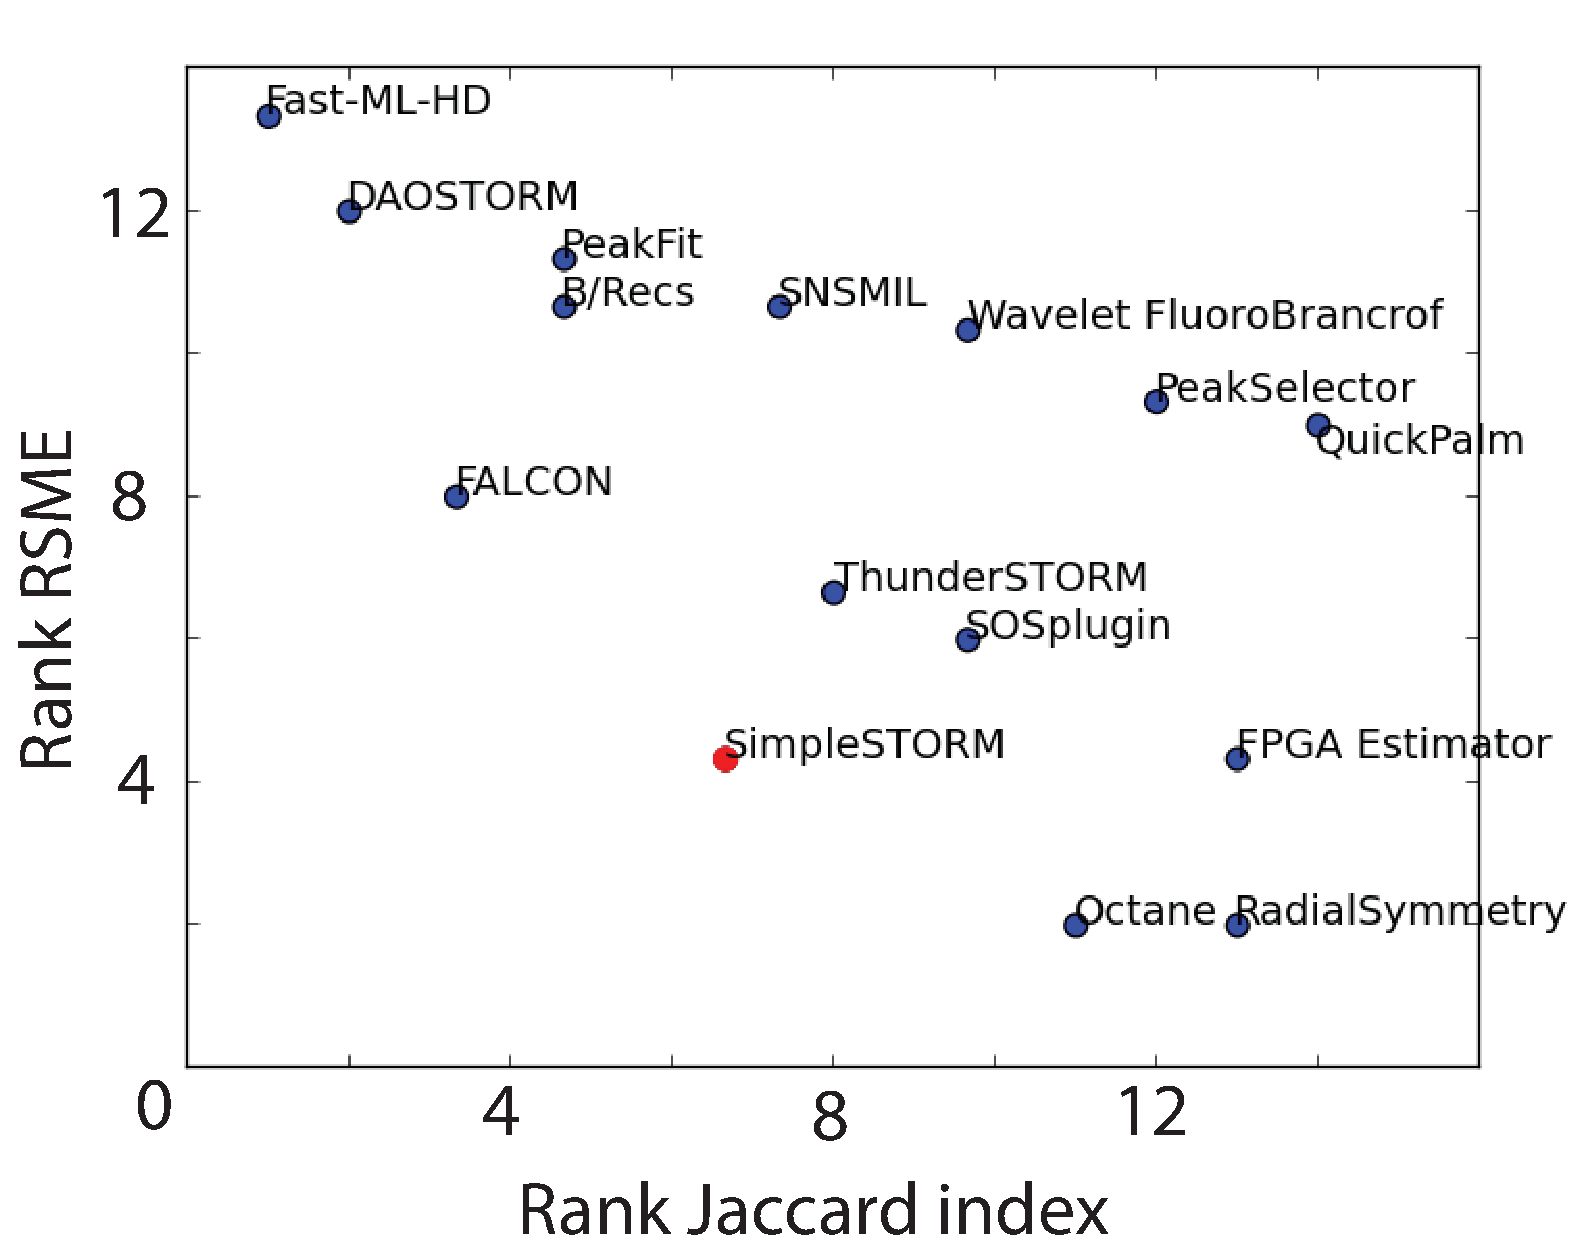
\includegraphics[width = 0.4\textwidth]{figures/high_Density_scatter.pdf}%
	\caption{Average algorithm rankings in the ISBI Localization Challenge (top: low density, bottom: high density datasets). Smaller distance to the origin is better.}%
	\label{scatterplot_challenge}%
\end{centering}
\end{figure}

Two of the training datasets show simulated tubulin tubes, and we will refer to them as `Tubulin 1' and `Tubulin 2'. They consist of 2400 frames with a resolution of 256 px * 256 px (at 150nm per pixel) and strong autofluorescent background. Tubulin 2 dataset has a higher noise level than tubulin 1. The other two datasets simulate a bundle of tubulin tubes. There is a long sequence with 12000 frames and almost no overlapping spots and a high density set with 361 frames and severely overlapping spots. These datasets will be referred to as `long sequence' (LS) and `high density' (HD) respectively. Both datasets consist of images with a resolution of 64 px * 64 px at 100 nm per pixel. Full details are available on the challenge web site.

In addition free program\footnote{\url{http://bigwww.epfl.ch/smlm/evaluation/index.html}} to compute performance metrics such as Jaccard index, F-score (both measuring detection reliability) and root mean square localization error (RMSE) accompanies the data.

\subsection{PSF Estimation}
We compared a non-parametric (Wiener filter) and two parametric (Gaussian fitting in the Fourier and spatial domains) algorithms for PSF estimation. The three estimation methods performed similarly on the test datasets with non-overlapping spots. This confirms that the Gaussian model is indeed applicable, because otherwise the Wiener filter would have been superior. Spatial domain fitting was slightly more robust than Fourier domain fitting, which tended to overestimate $\sigma_{\psf}$ and occasionally failed to converge to the correct solution. Since a Gaussian matched filter is faster than a Wiener filter, we prefer the former. Figures \ref{histogram_of_sigmas} (a-d) show the distribution of sigmas estimated by applying the Levenberg-Marquardt algorithm to all spots in the first 2000 frames (respectively all frames in the high density dataset). The full width at half maximum (FWHM) of the true PSF was 258~nm in all cases, which translates into $\sigma_{\mathrm{true}}=0.73$ pixels in Tubulin 1 and 2 and into $\sigma_{\mathrm{true}}=1.09$ pixels in the others. Our estimate of $\sigma_{\psf}$ is the median of these histograms and within $10\%$ of the true values, except in the high density dataset where our estimate is slightly too high because the fitting algorithm falsly merged  some overlapping spots. 
\begin{figure}
\subfloat[Tubulin 1 dataset]{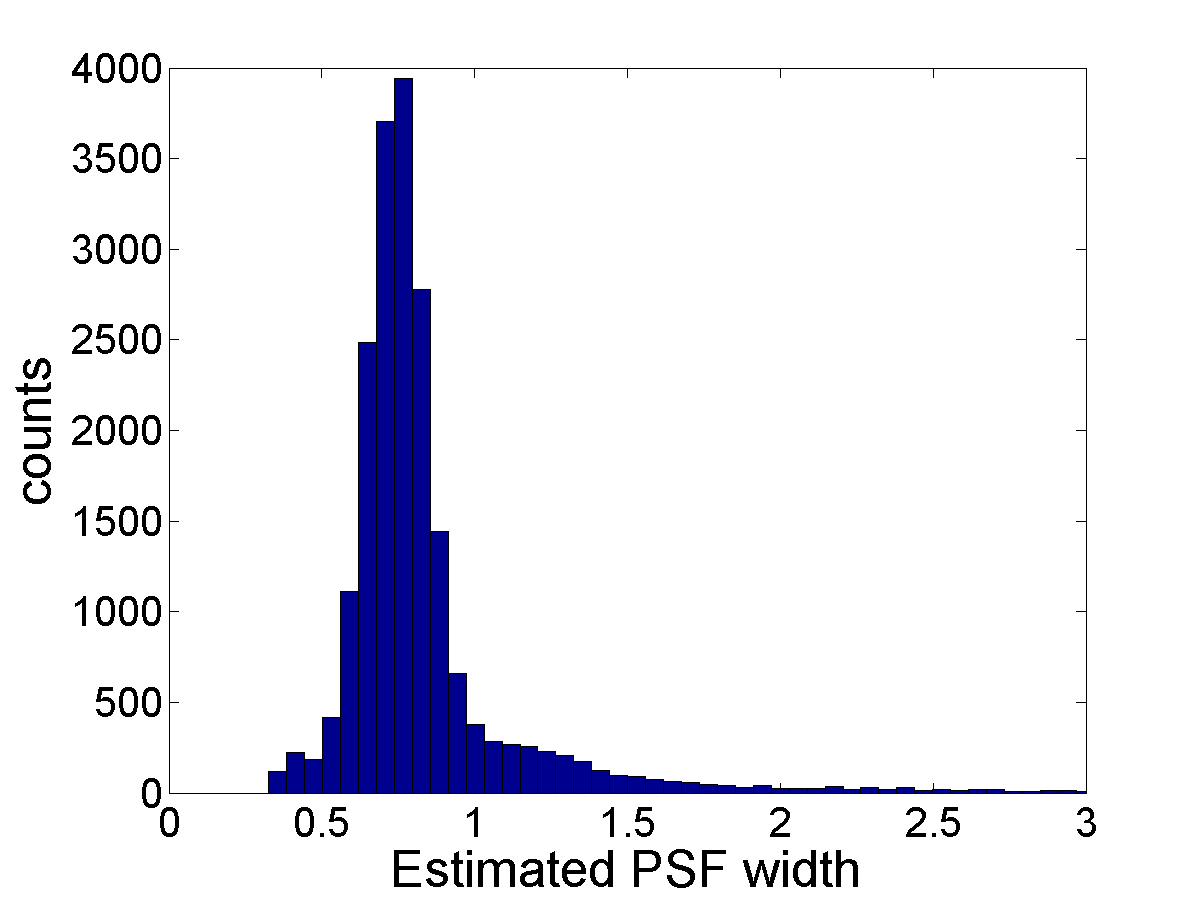
\includegraphics[width = 0.24\textwidth]{figures/SigmaTubulin1.png}}\hfill%
\subfloat[Tubulin 2 dataset]{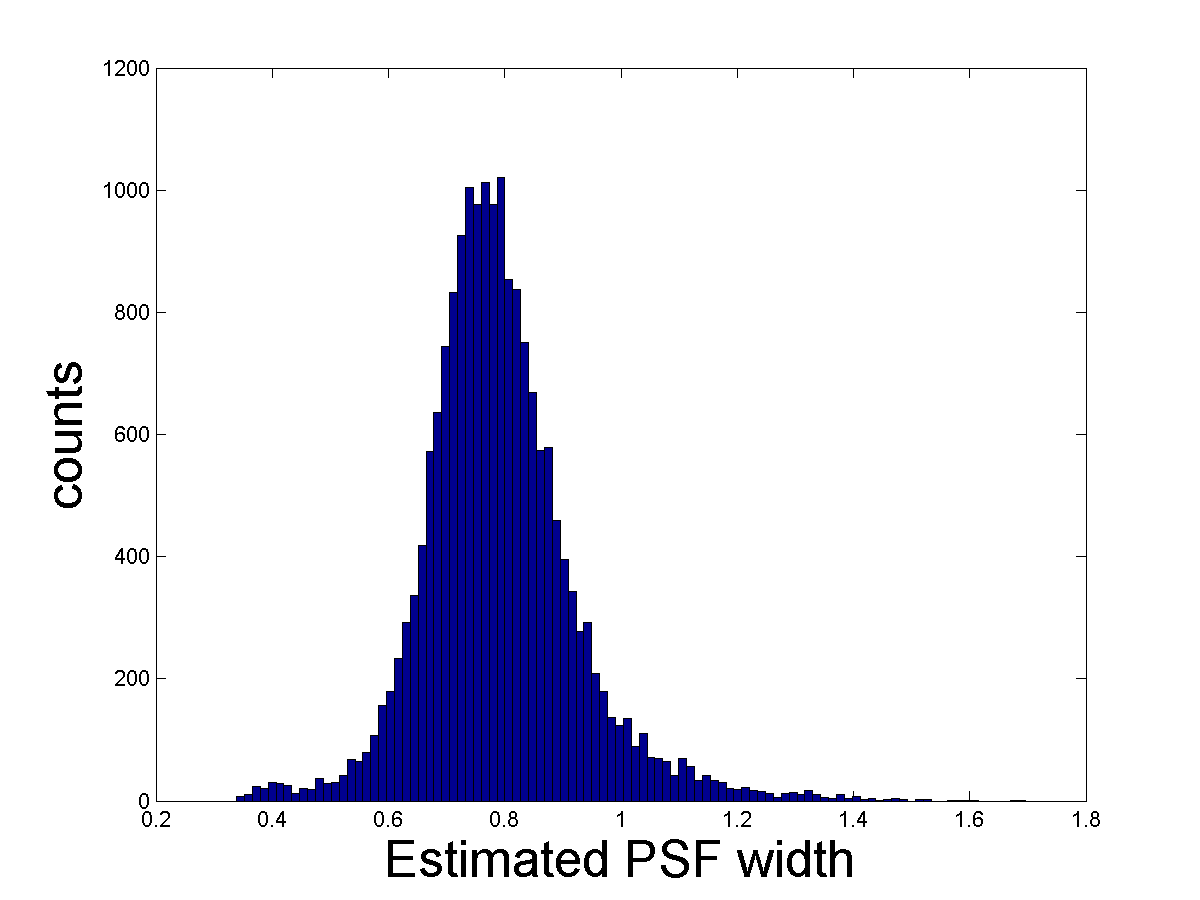
\includegraphics[width = 0.24\textwidth]{figures/SigmaTubulin2.png}}\\
\subfloat[Long sequence dataset]{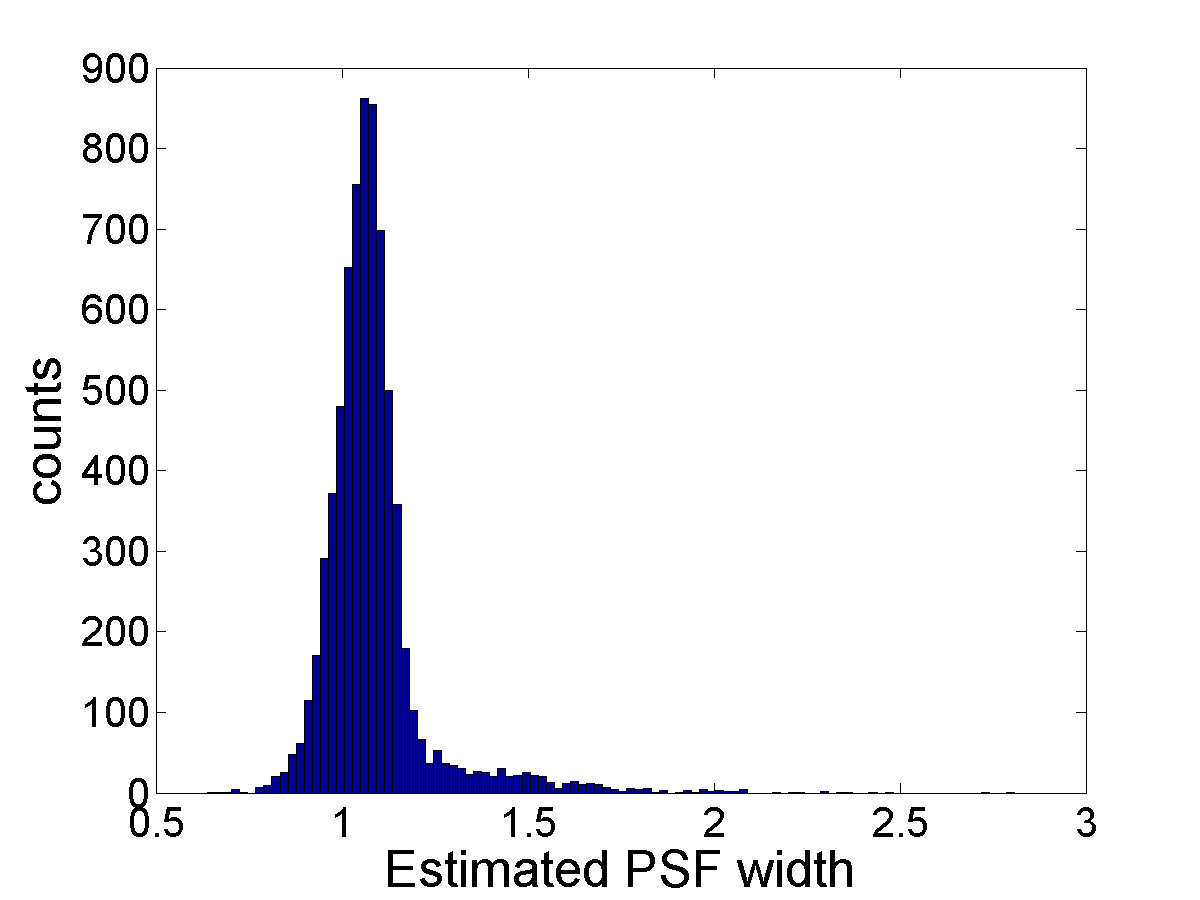
\includegraphics[width = 0.24\textwidth]{figures/SigmaBundledTubes1.png}}\hfill%
\subfloat[High density datase]{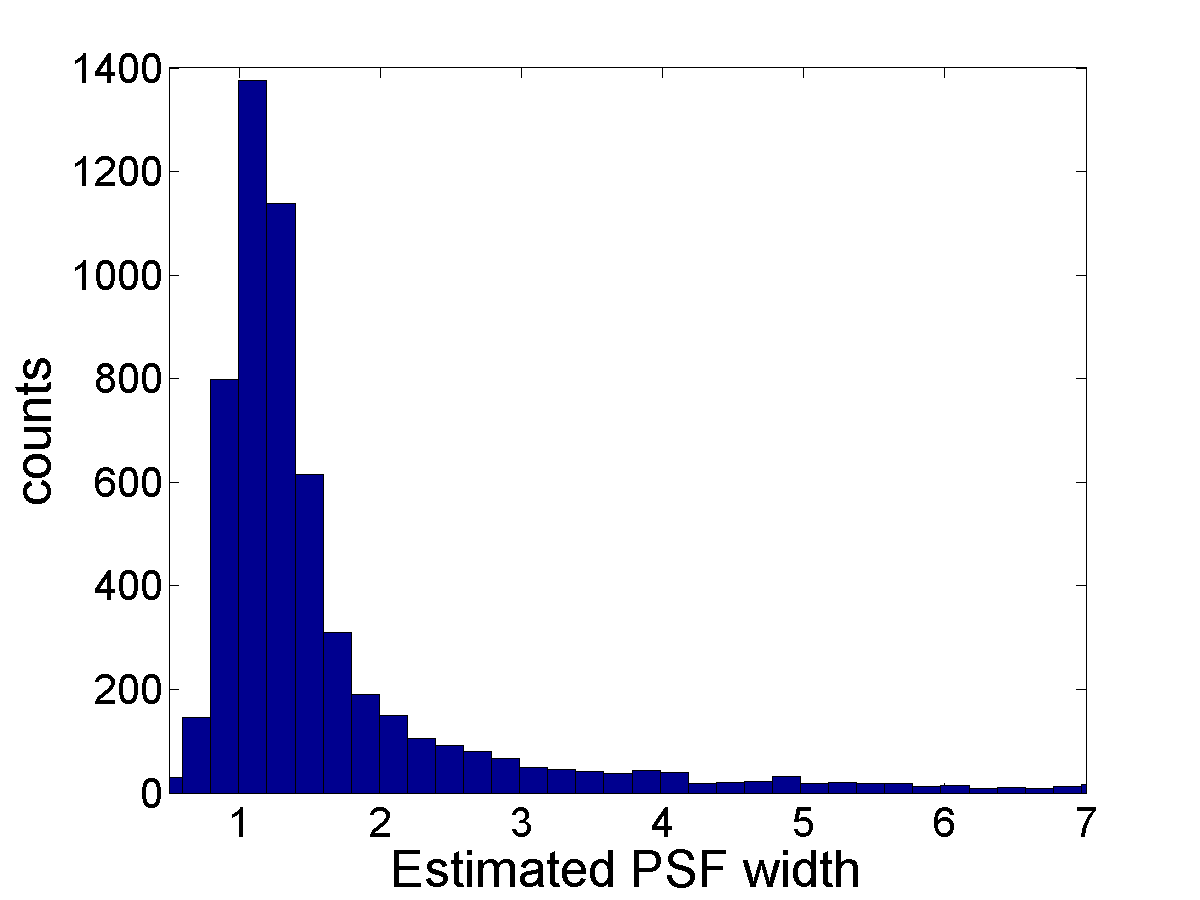
\includegraphics[width = 0.24\textwidth]{figures/SigmaBundledTubes2.png}}%
	\caption{Histograms of estimated $\sigma_{\psf}$ for the training datasets from the ISBI localization challenge}%
	\label{histogram_of_sigmas}%
\end{figure}

To improve results in high density datasets, another advantage of the parametric PSF model comes into effect: It is easy to change the filter strength by choosing $\sigma_{\mathrm{filter}}<\sigma_{\psf}$. This reduces the tendency of overlapping spots to be erroneously fused. Figure \ref{sigmas_quantitative} shows the RMSE as a function of $\sigma_{\mathrm{filter}}$ for low and high density data. It can be seen that the matched filter indeed minimizes the RMSE when spots do not overlap, whereas the optimal filter size is much smaller when spots overlap. The same effect is illustrated qualitatively in figure \ref{sigmas}: The detection quality clearly decreases with increasing $\sigma_{\mathrm{filter}}$. Therefore, we choose a small value for $\sigma_{\mathrm{filter}}$ for high density data.
\begin{figure}
\subfloat[Low density dataset]{
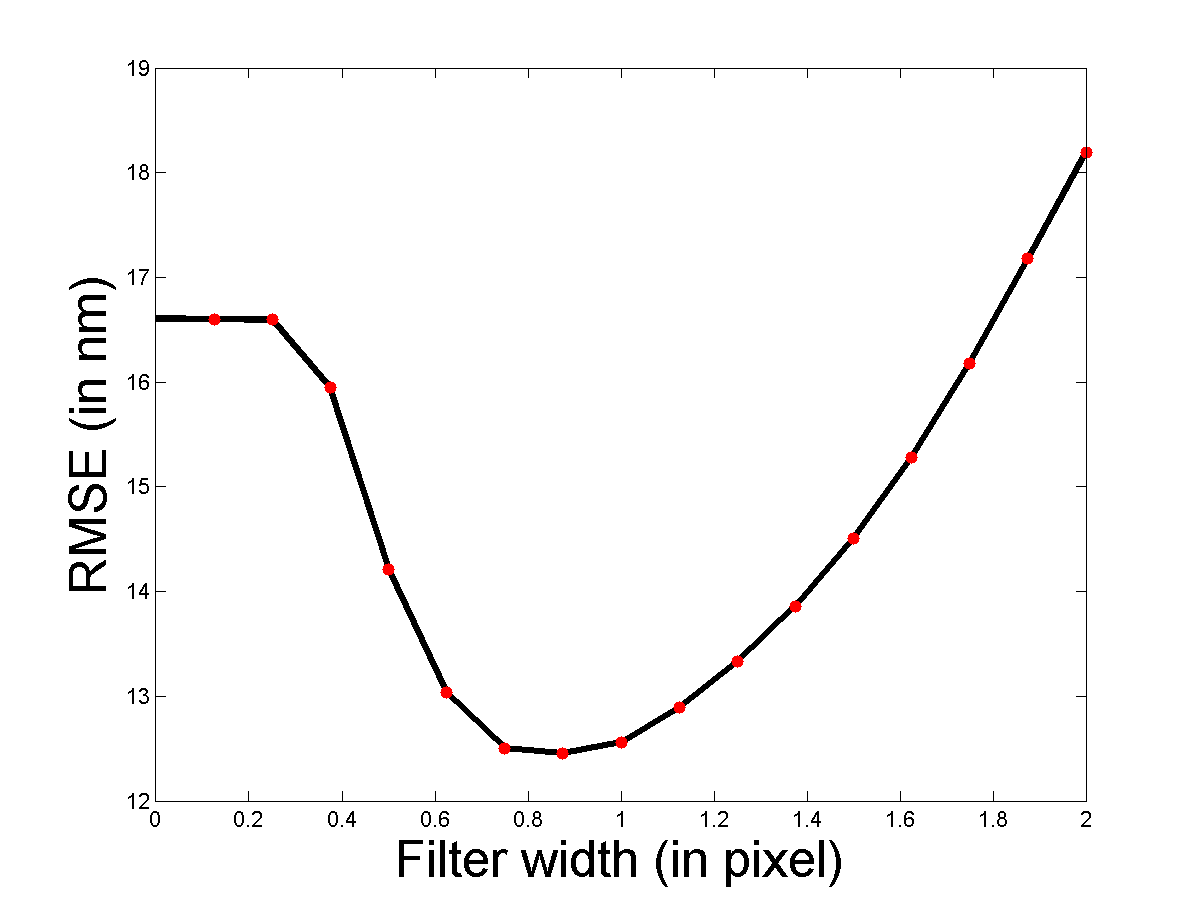
\includegraphics[width=0.23\textwidth]{figures/RMSE_filterwidthLD.png}\label{sigmas_quantitativeA}}\hfill%
\subfloat[High density dataset]{
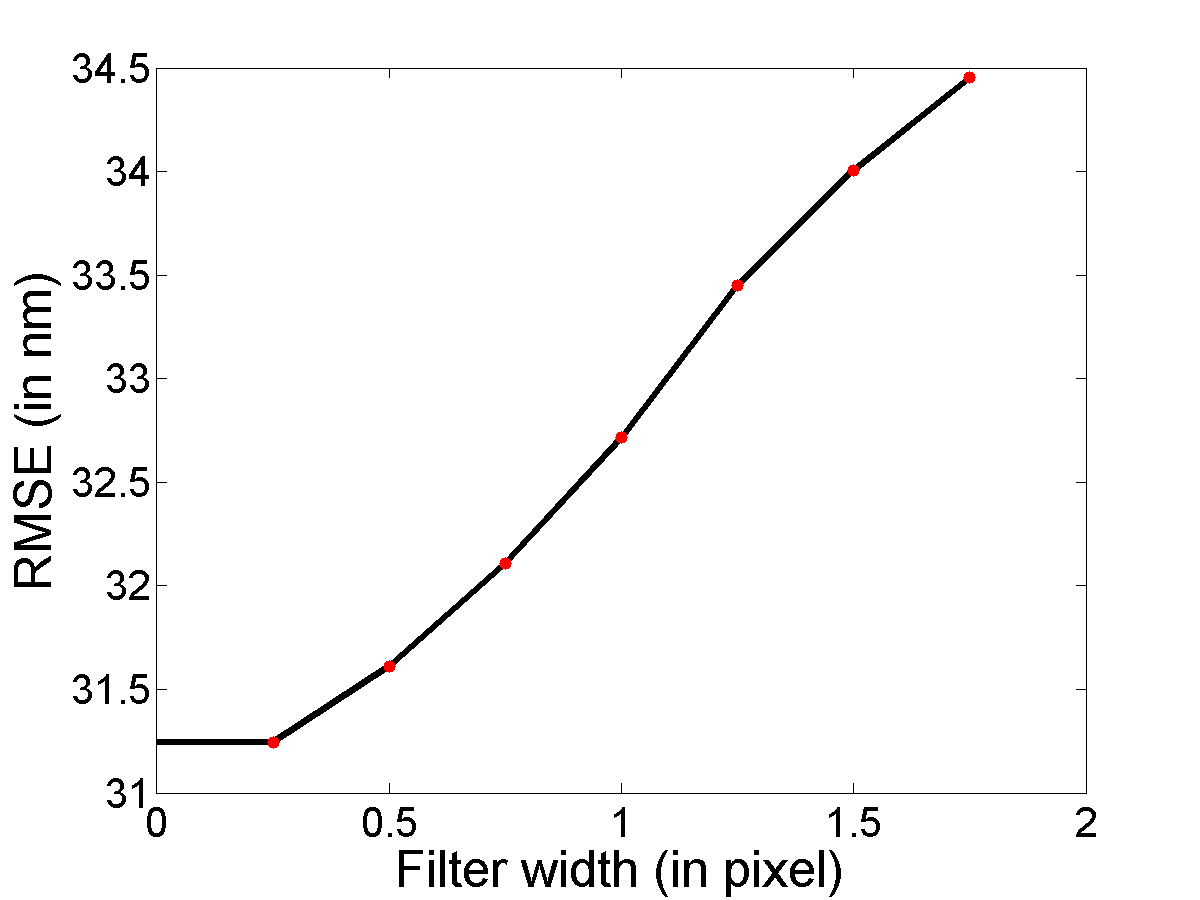
\includegraphics[width=0.23\textwidth]{figures/RMSE_filterwidthHD.png}\label{sigmas_quantitativeB}}
	\caption{RMSE for different filter widths.}%
	\label{sigmas_quantitative}%
\end{figure}
\begin{figure}
\subfloat[$\sigma = 0$]{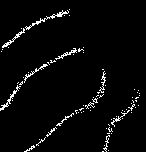
\includegraphics[width = 0.15\textwidth]{figures/bundledTubulins2_sigma_0_croped2.png}}\hfill%
\subfloat[$\sigma = 1$]{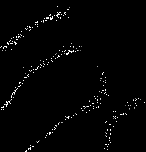
\includegraphics[width = 0.15\textwidth]{figures/bundledTubulins2_sigma_1_croped2.png}}\hfill%
\subfloat[$\sigma = 1.5$]{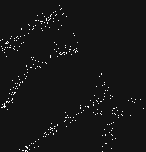
\includegraphics[width = 0.15\textwidth]{figures/bundledTubulins2_sigma_1_5_croped2.png}}\hfill%
	\caption{The effect of filter width on high density data.}%
	\label{sigmas}%
\end{figure}

\subsection{Gain estimation}
A key feature of SimpleSTORM is the estimation of the camera gain directly from the data. This is important since the actual gain factor differs from the value indicated by the camera's  control settings. For validation purposes, we captured a series of 500 frames of a standard cell culture with phalloidin labeled actin filaments using different gain settings in the camera. Figure \ref{gain_verification} shows that the true and indicated gain values differ, but are proportional to each other. This justifies our linear model (\ref{eq:linear-gain-model}) and the gain estimation method of section \ref{sec:noise-normalization}.
\begin{figure}
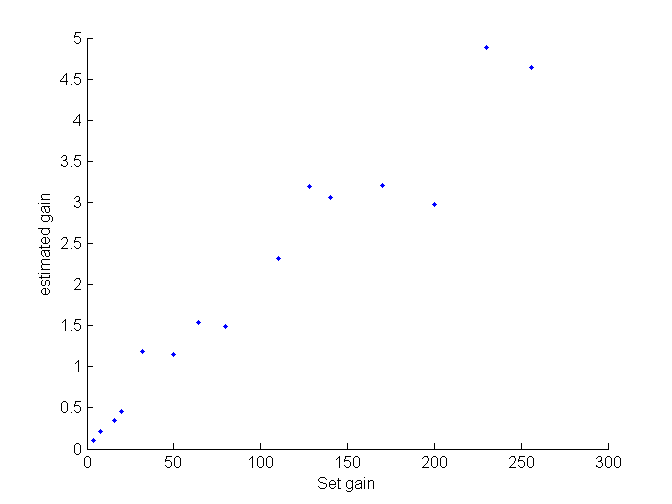
\includegraphics[width=0.45\textwidth]{figures/gain_estimation}
\caption{Scatter plot of estimated gain vs. gain setting in the camera.}
\label{gain_verification}
\end{figure}

\subsection{Image standardization} \label{bg_estimation}
To check whether the image standardization works as desired, we measure the false positive rate of the statistical test according to section \ref{sec:spot-detection} on the image background. Since the ground truth is known, we can define the background precisely as the set of pixels which are at least 4 pixels away from any true spot position. For the plain statistical test (without connectivity constraint), the false positive rate should equal the $p$-value. To verify this, we counted the fraction of background pixels whose intensity exceeds the threshold according to (\ref{eq:detection-threshold}) after image standardization. Figure \ref{fp_rate} shows results for Tubulin 1 where the actual error rate is even a bit less than expected. As can be seen in figure \ref{fp3_rate}, the additional connectivity test reduces the error rate further: Out of 46 million background pixels, we found 228 false positives for $p=1\%$ and only 16 for $p=0.1\%$.
\begin{figure}
\subfloat[without connectivity test]{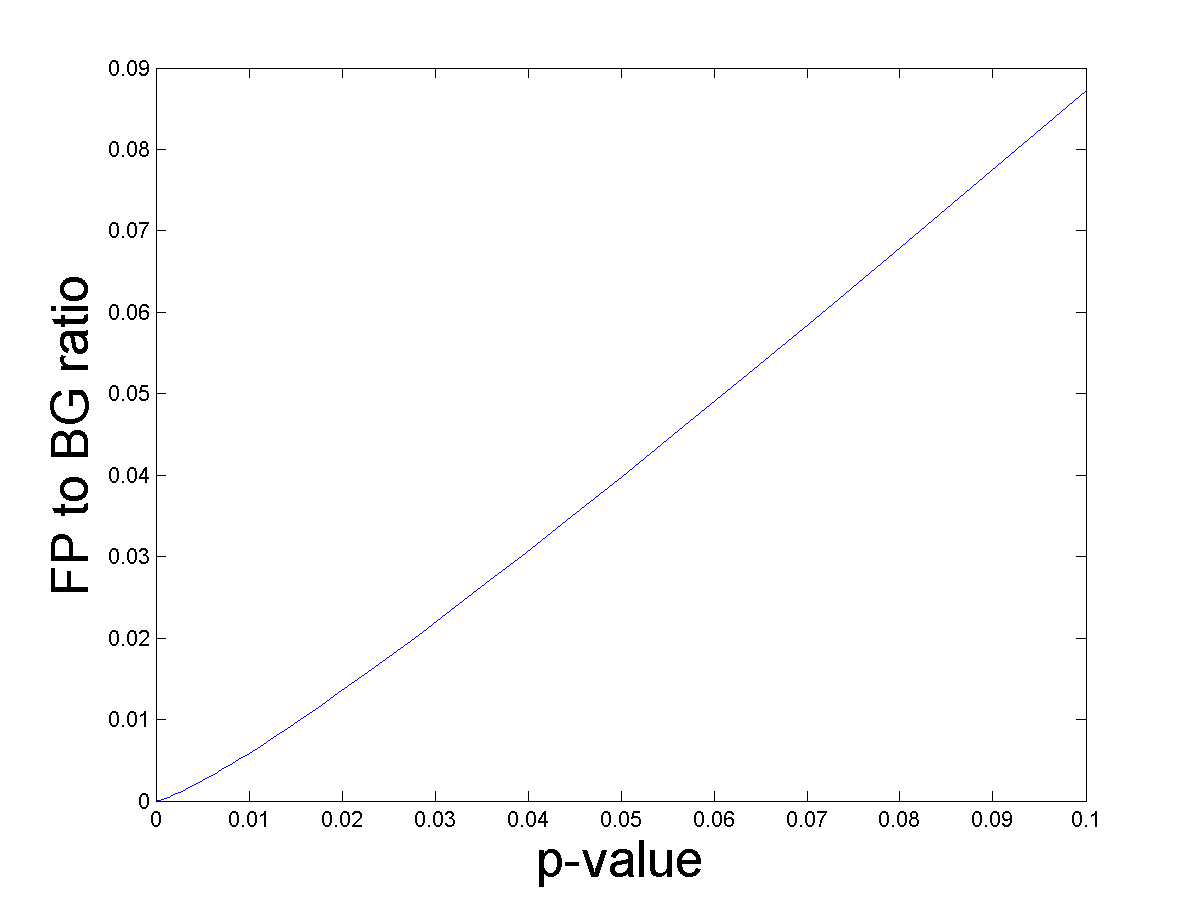
\includegraphics[width = 0.24\textwidth]{figures/FP_BgRatioTubulin1.png}\label{fp_rate}}\hfill%
\subfloat[with connectivity test]{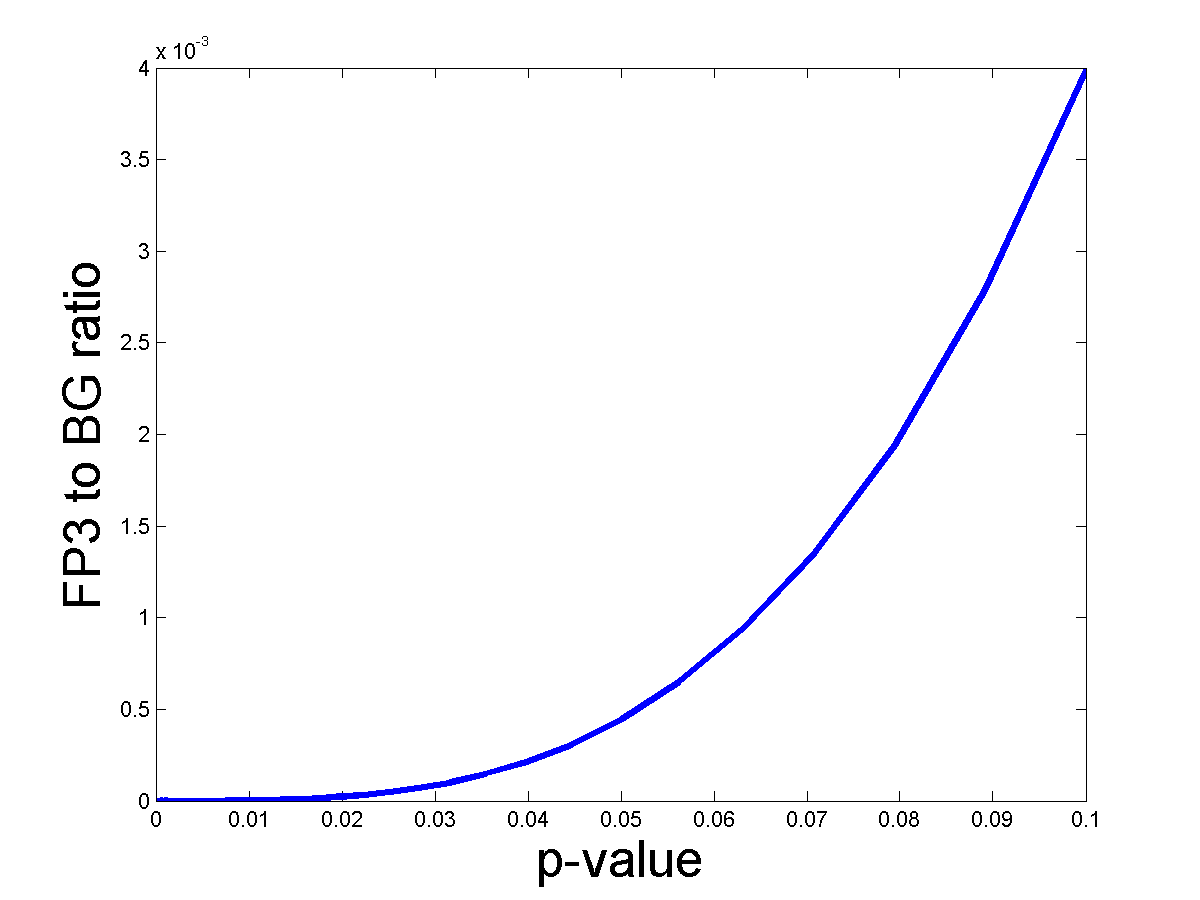
\includegraphics[width = 0.24\textwidth]{figures/FP3_BgRatioTubulin1.png}\label{fp3_rate}}\hfill%	
\caption{False positives rates for Tubulin 1 as a function of $p$.}%
\end{figure}

\subsection{Reconstruction results}

We finally report results for the entire SimpleSTORM algorithm on artificial and real data. For the artificial data, we adopt the performance metrics suggested by the ISBI challenge, namely the {\em Jaccard index}
\[
\mathrm{Jaccard}=\frac{\mathrm{TP}}{\mathrm{FN}+\mathrm{TP}+\mathrm{FP}}
\]
the F-score which is defined via precision and recall as
\begin{eqnarray*}
\mathrm{Recall:}\quad &\mathrm{R}=&\frac{\mathrm{TP}}{\mathrm{TP}+\mathrm{FN}}\\
\mathrm{Precision:}\quad &\mathrm{P}=&\frac{\mathrm{TP}}{\mathrm{TP}+\mathrm{FP}}\\
\mathrm{F-score:}\quad &\mathrm{F}=&\frac{2\,\mathrm{R}\,\mathrm{P}}{\mathrm{R}+\mathrm{P}}\\
\end{eqnarray*}
and the root mean square error
\[
\mathrm{RMSE}=\left(\frac{1}{\mathrm{TP}}\sum_{i=1}^{\mathrm{TP}}d(\vec{x}_i^*,\vec{x}_i)^2\right)^{1/2}
\]
where $\mathrm{TP}$, $\mathrm{FN}$, and $\mathrm{FP}$ are the number of true positives, false negatives and false positives respectively, and $d(\vec{x}_i^*,\vec{x}_i)$ is the Euclidean distance of the $i^{\mathrm{th}}$ detection from the corresponding ground truth location. A true match is recorded if the ground truth position is within radius $r$ of the detection, and each ground truth point can be assigned at most once. We use the evaluation tool from the ISBI challenge website to compute these metrics with $r=0.3\mathrm{px}$. 

Table \ref{result_Training_0_3} shows the metrics and the processing speed for the four training data\-sets, where SimpleSTORM was run with standard settings on the first three datasets. That is, gain, offset, and PSF size were determined by self-calibration, the $p$-value was set to 0.01\%, and the reconstructed images were 8-fold upsampled relative to the originals. In the high density dataset, matched filtering was skipped, and an asymmetry threshold of 2 was introduced. Corresponding reconstructions are shown in figures \ref{tubulin1} and \ref{highdensity}. The reconstructed images contain both our detections and ground truth. It can be seen in the low density dataset (figure \ref{tubulin1} right) that the detections are typically within one pixel of the ground truth position in the reconstructed image. On the difficult high density dataset, SimpleSTORM still performs reasonably after the indicated manual parameter adjustments. While these adjustments result in a rather low recall, the localization error of the surviving spots is acceptably low.  In addition table \ref{result_Training_0_3} also contains the performance of rapidSTORM (version 3.2) with settings adjusted to yield approximately the same quality than SimpleSTORM. For big data sets rapidSTORM processes the data  5 to 6 times faster than SimpleSTORM. For small data sets it depends on the number of frames, rapidSTORM performed up to 11 times better for the long sequence data set with 12000 frames.

\begin{table}
\caption{SimpleSTORM performance }
\tabcolsep=0.11cm
\begin{tabular}{l|ccccccc}
&&&&\multicolumn{2}{c}{frames per sec}\\
&Jaccard&Precision&RMSE&SimpleST.& rapidST.\\ \hline
Tubulin1&0.437&0.936&15.7\,nm&51&333\\
Tubulin2&0.232&0.904&18.8\,nm&72&387\\
LS&0.761&0.946&9.97\,nm&563&6000\\
HD&0.031&0.449&20.55\,nm&257&257
\end{tabular}
\label{result_Training_0_3}
\end{table}
\begin{figure*}
\begin{centering}
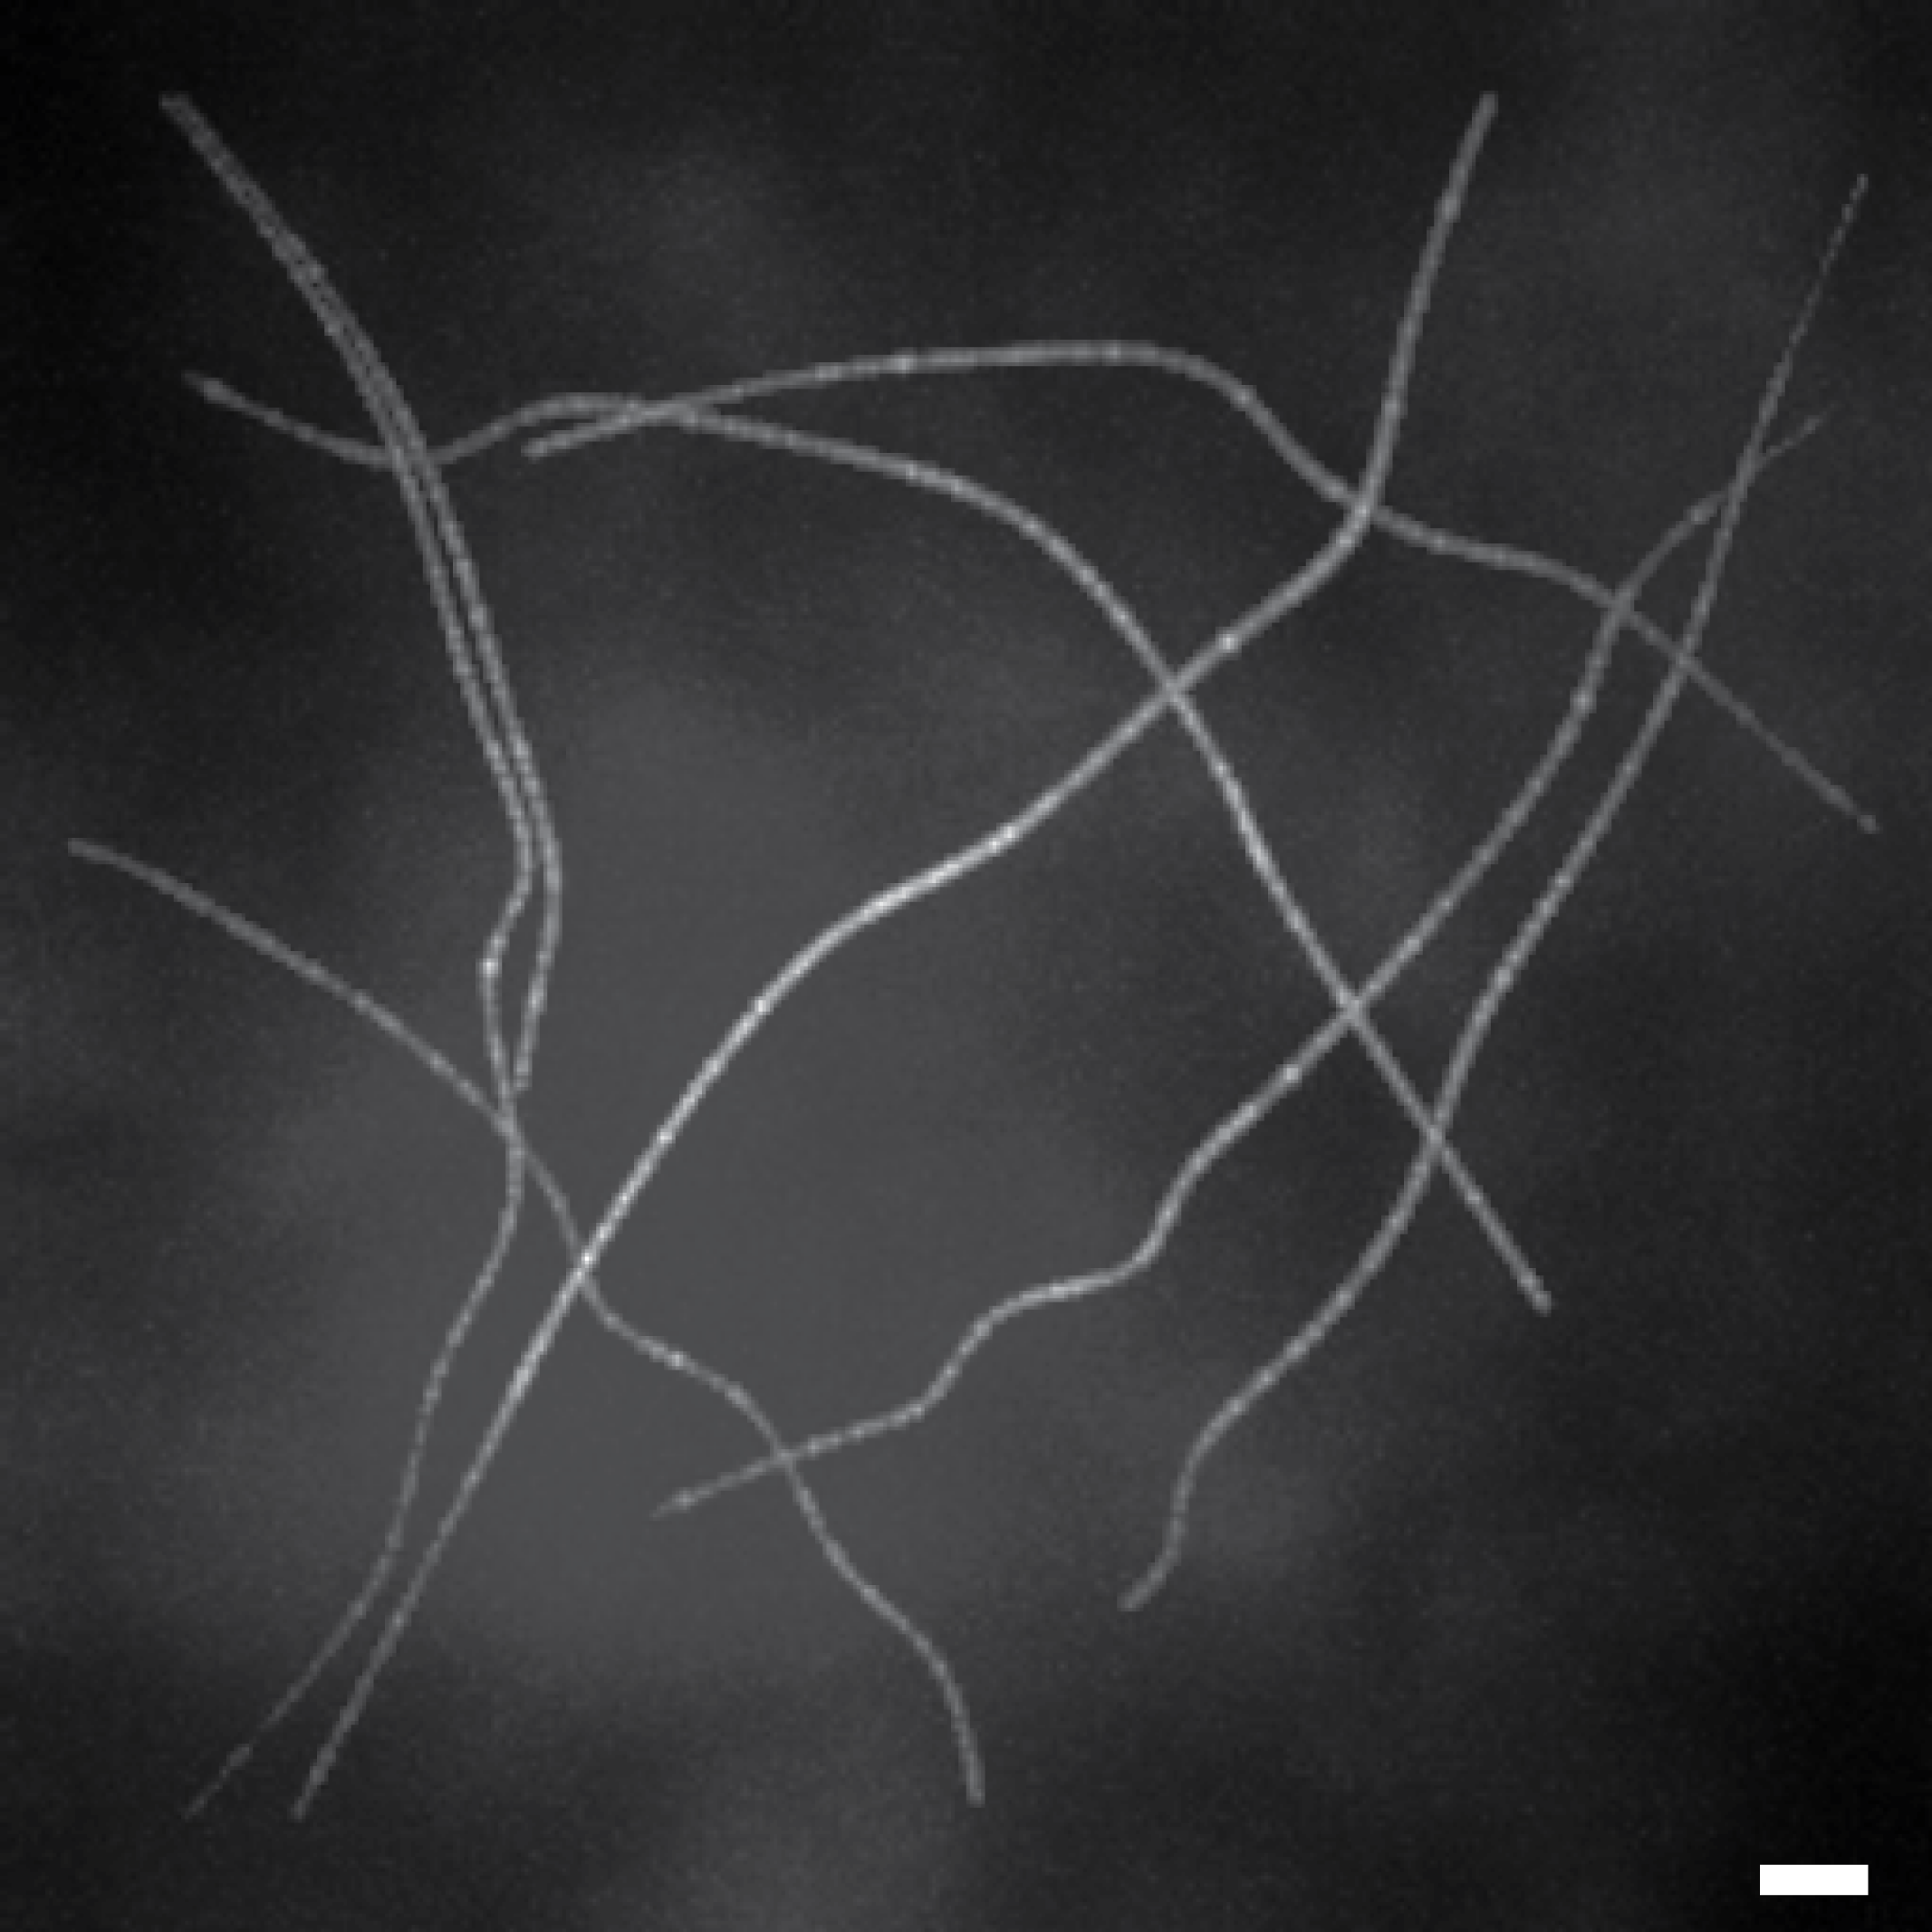
\includegraphics[width=0.3\textwidth]{figures/Tubulin1_zproj_scalebar.png}$\qquad$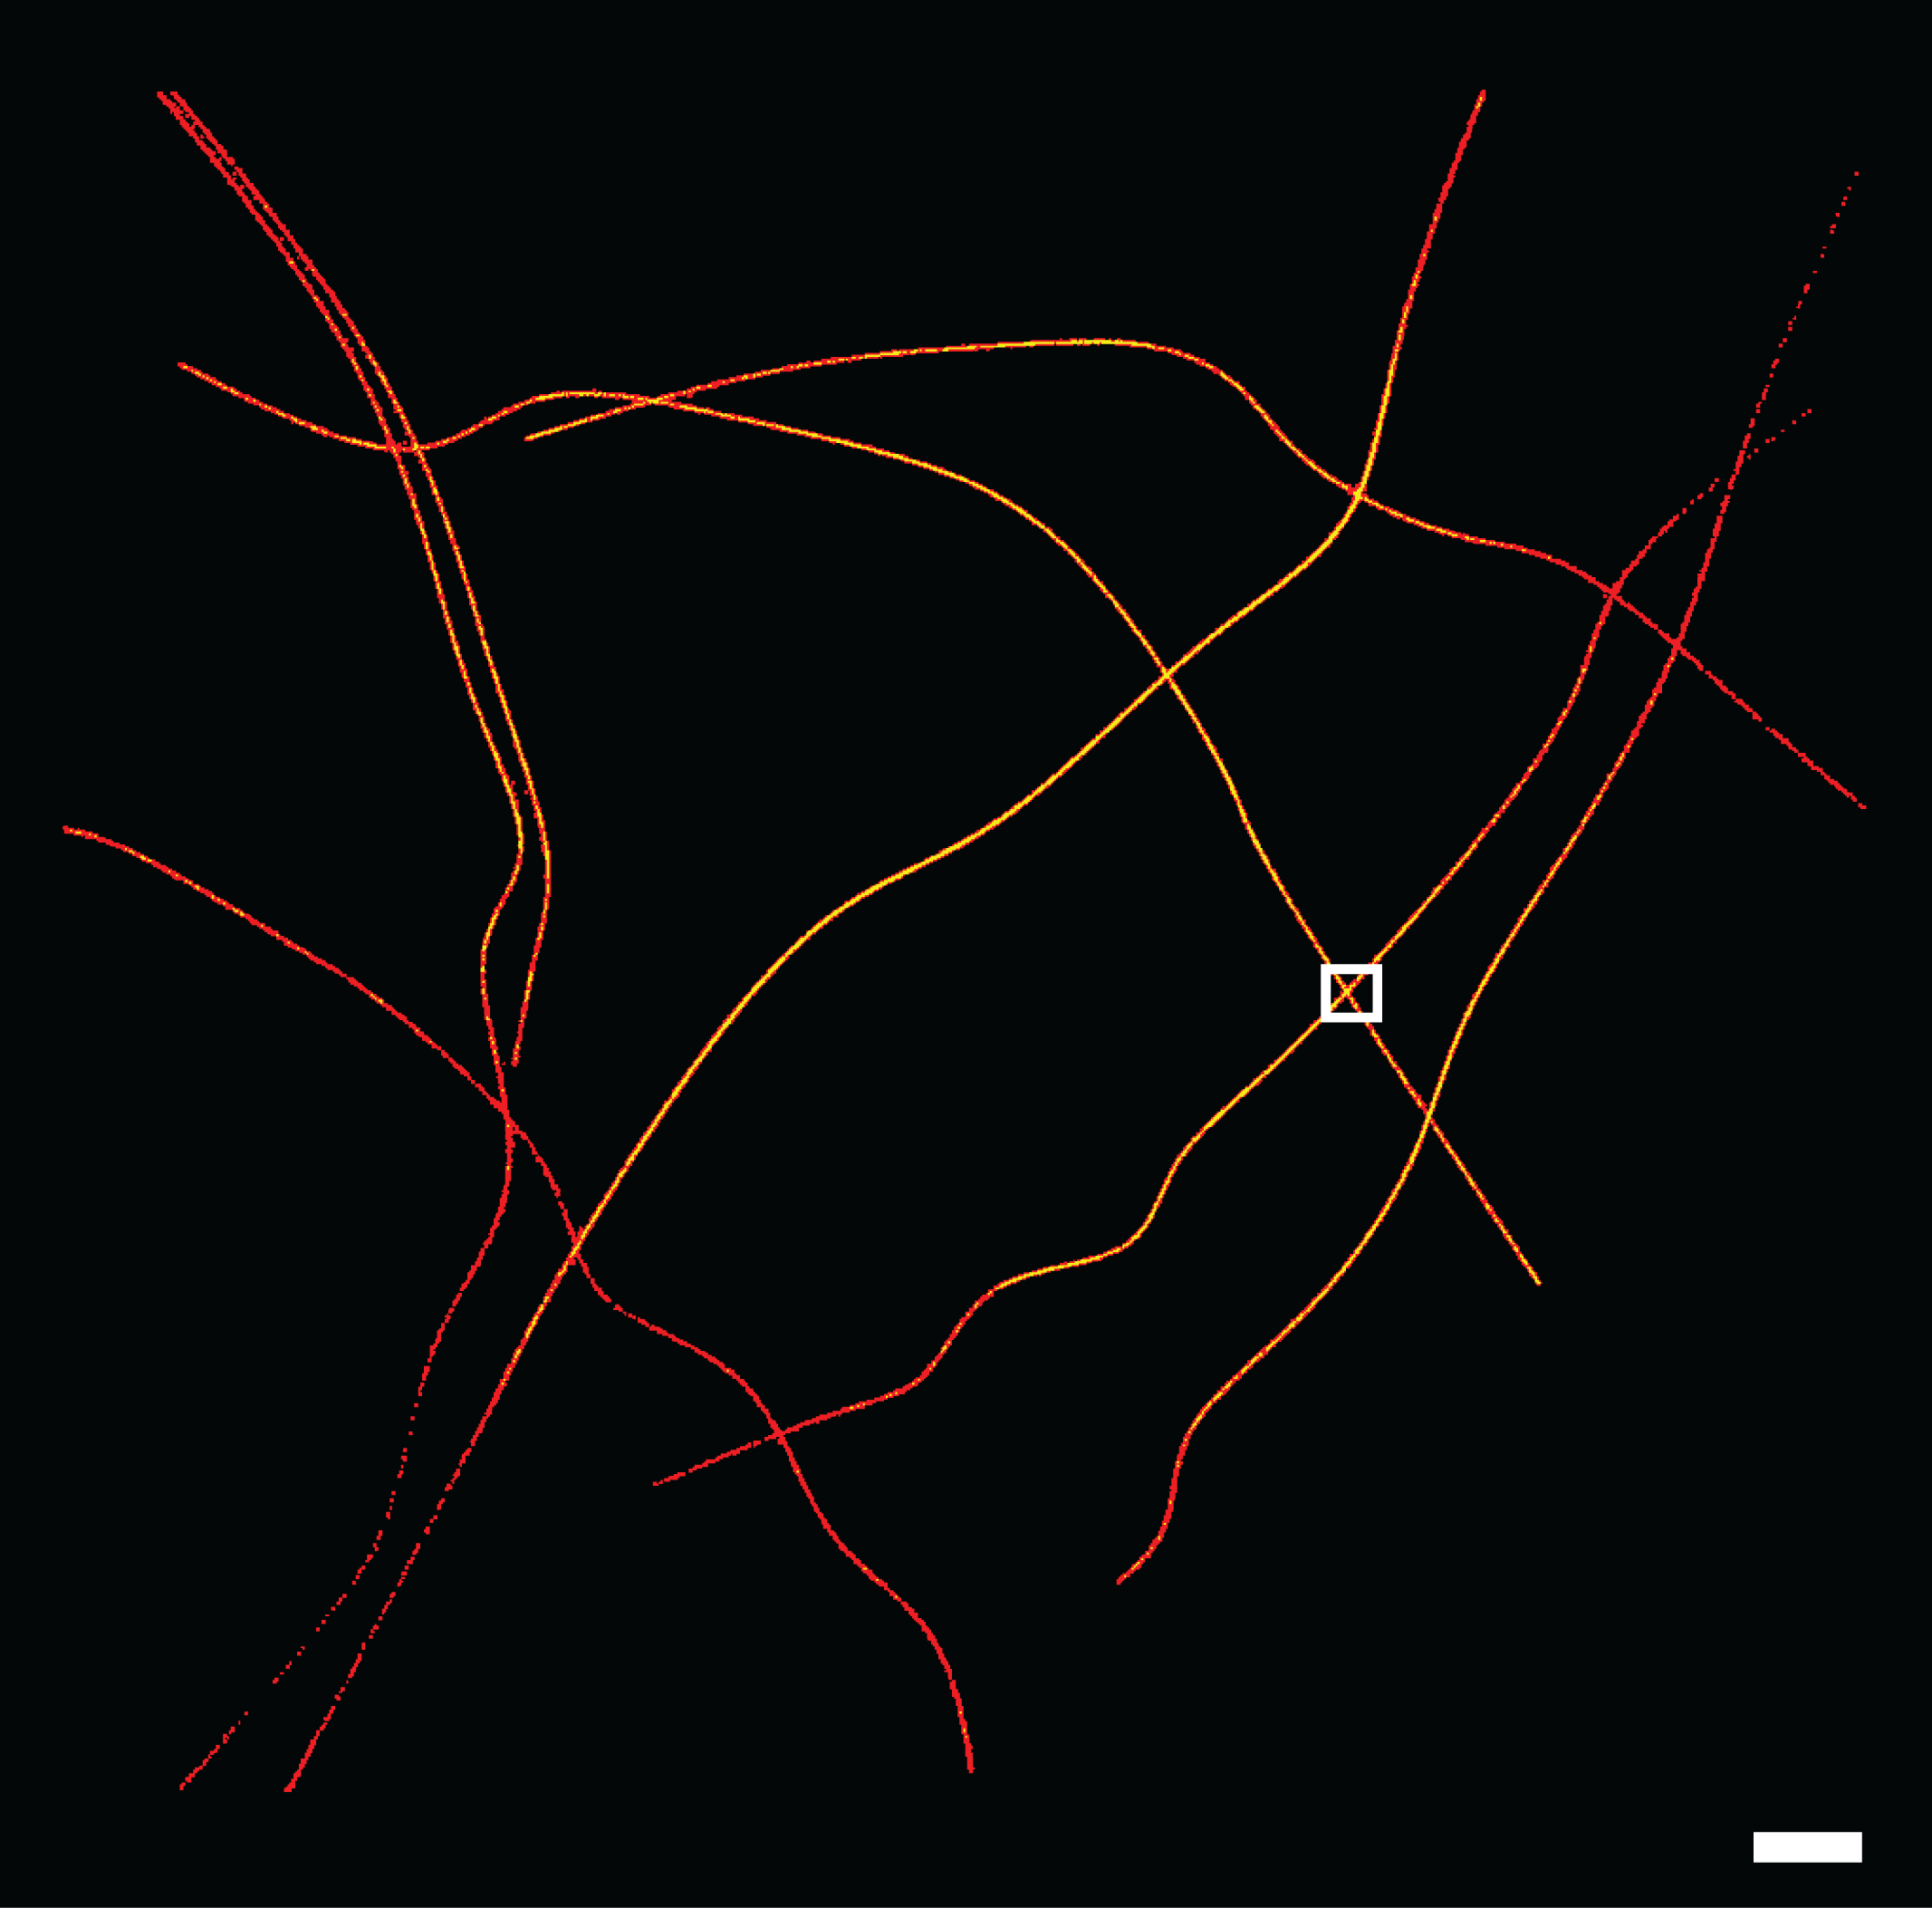
\includegraphics[width=0.3\textwidth]{figures/Tubulin1_reconstructed_rect2_hc_scalebar.png}$\qquad$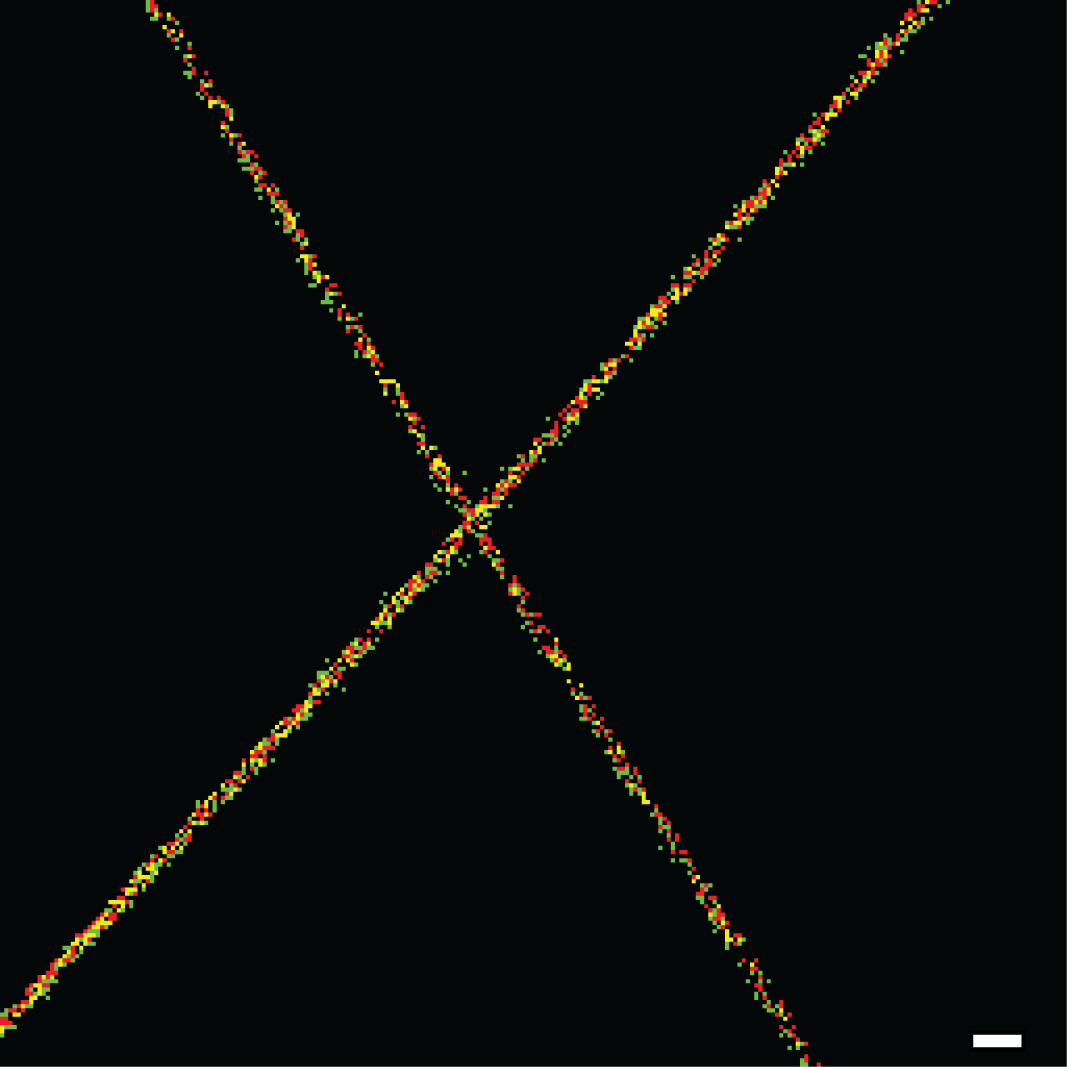
\includegraphics[width=0.3\textwidth]{figures/Tubulin1_ausschnitt2_scalebar.png}
\par\end{centering}

\caption{Tubulin 1. Left: mean projection of the raw data. Center: reconstructed image. Right: localizations (green) and ground truth (red), yellow indicates perfect alignment. Scalebar represents $2\,\mu m$ for the first two images and 100\,nm for the third.}\label{tubulin1}
\end{figure*}
\begin{figure*}
\begin{centering}
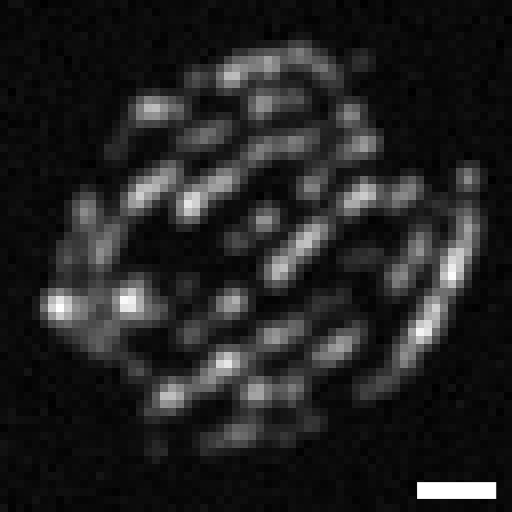
\includegraphics[width=0.3\textwidth]{figures/high-density_003.png}$\qquad$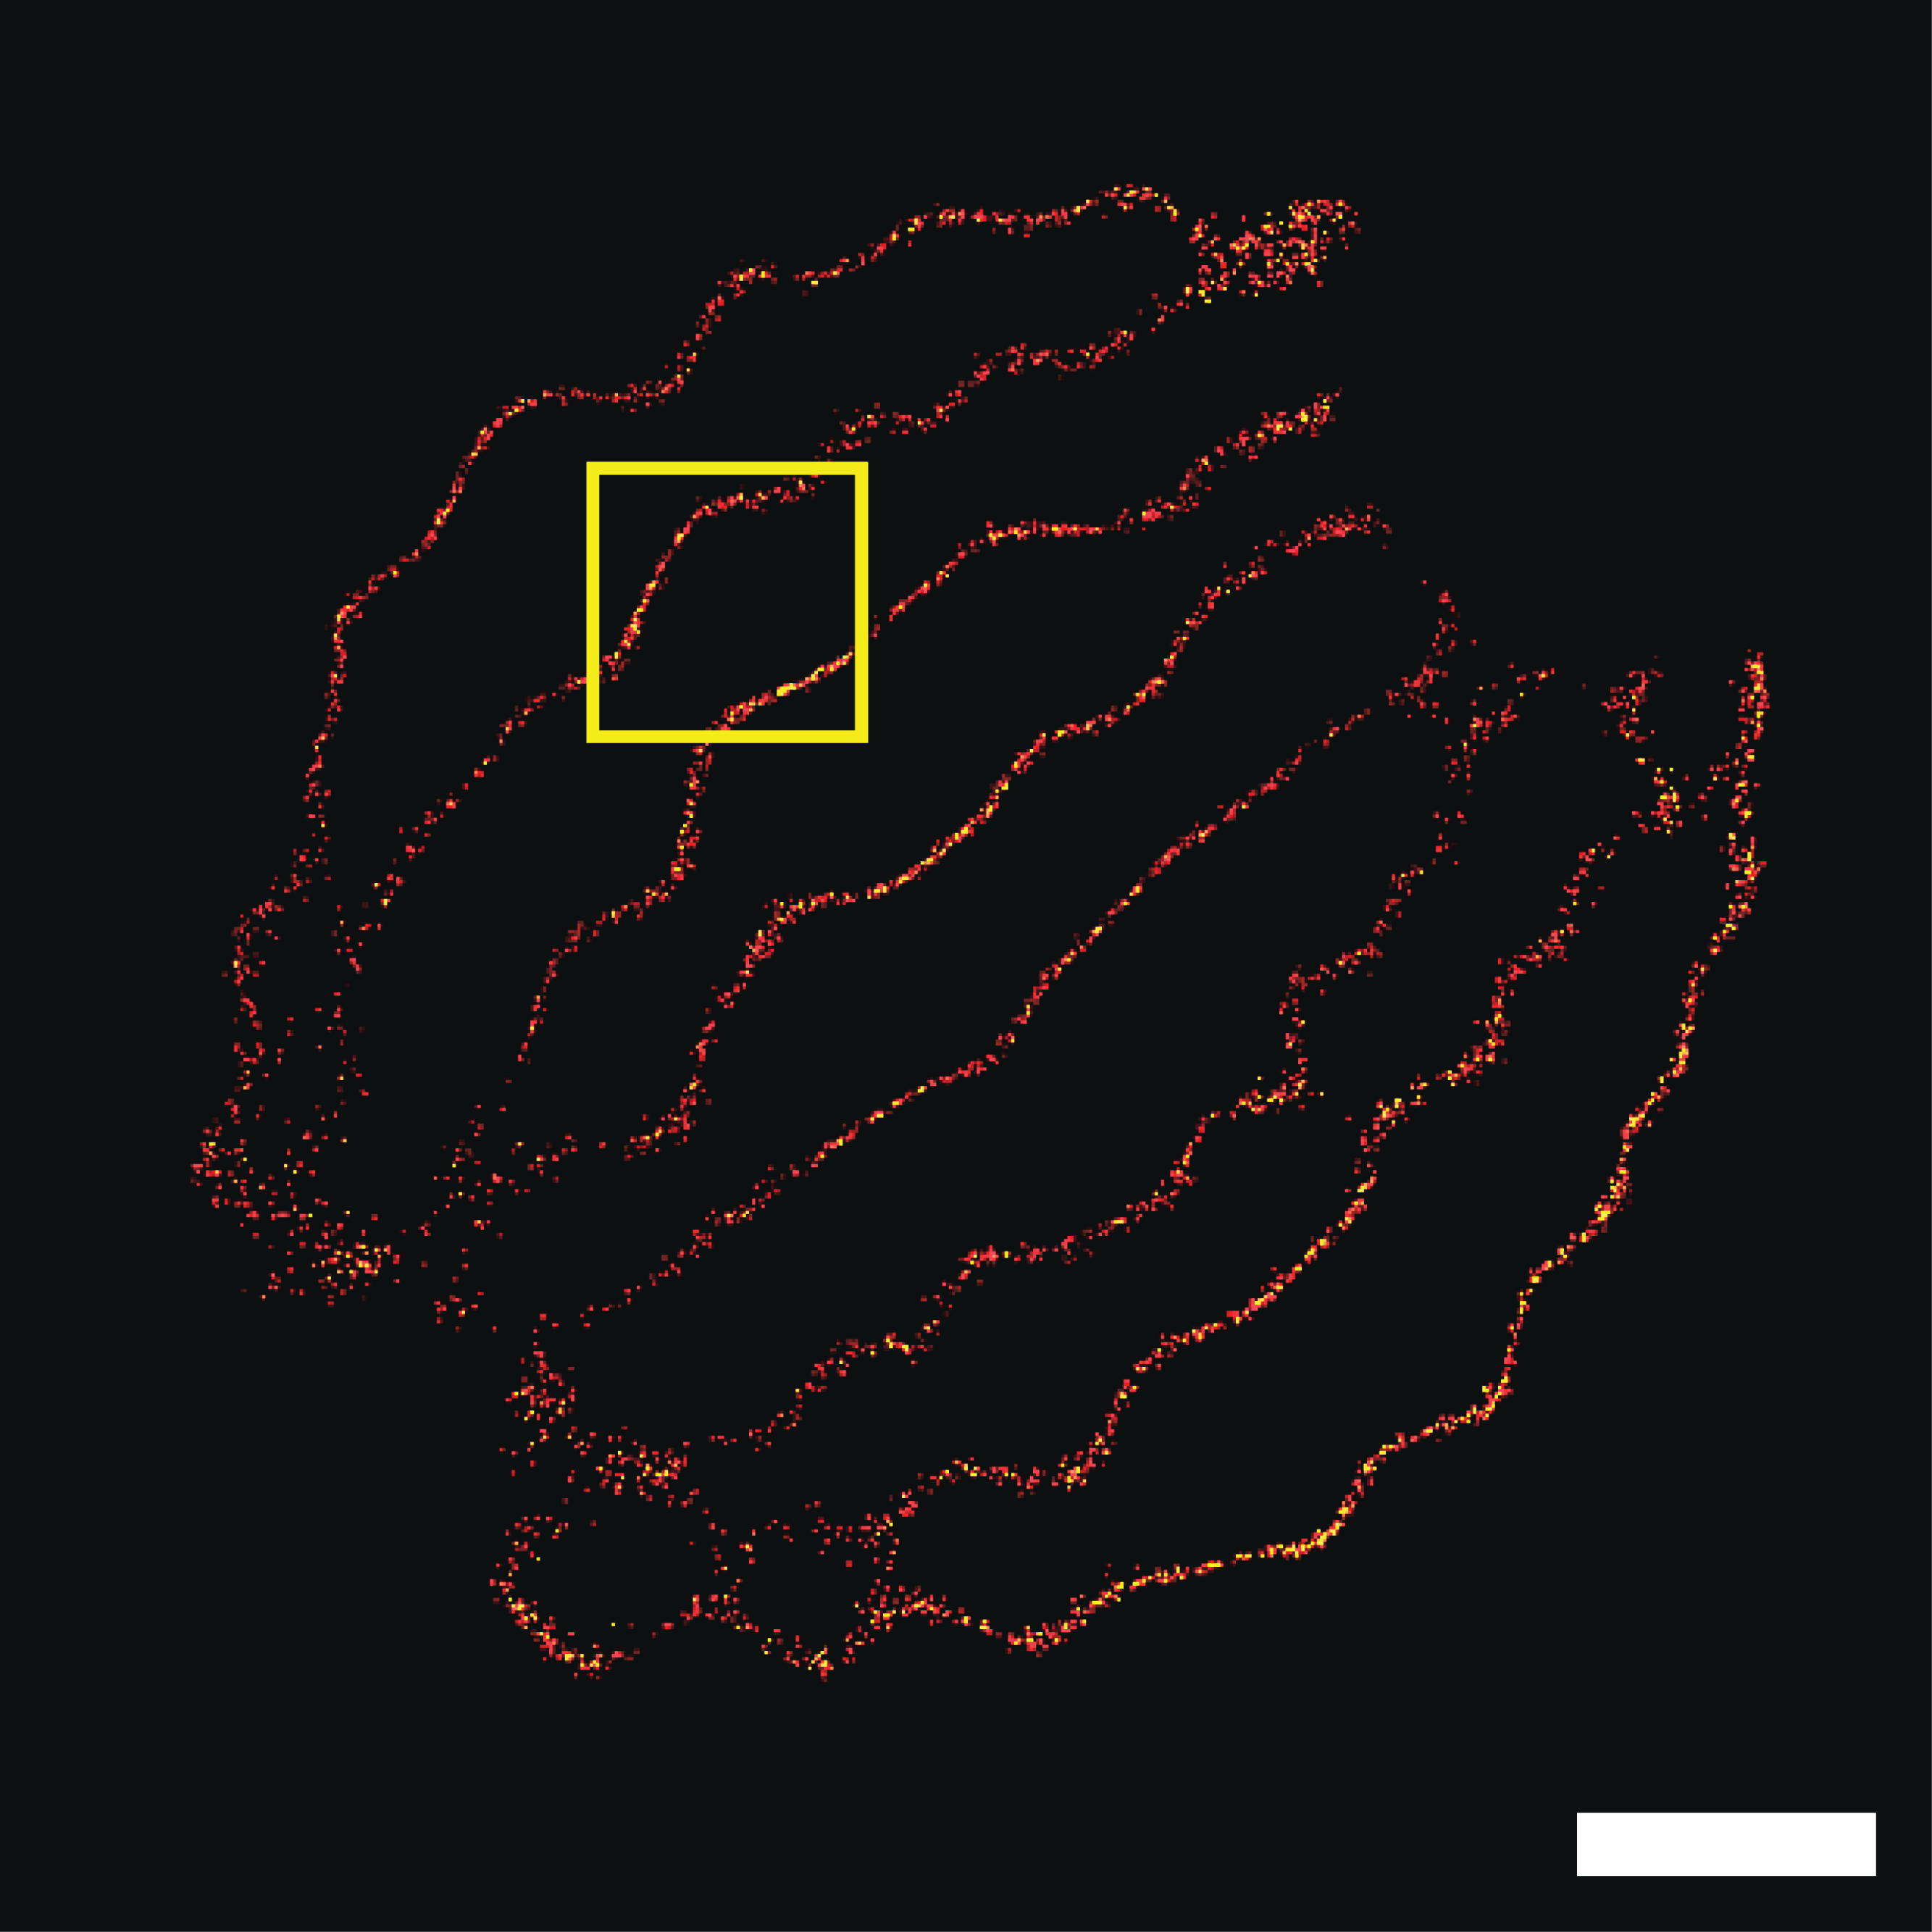
\includegraphics[width=0.3\textwidth]{figures/highdensityreconstruction_rect_hc_scalebar.png}$\qquad$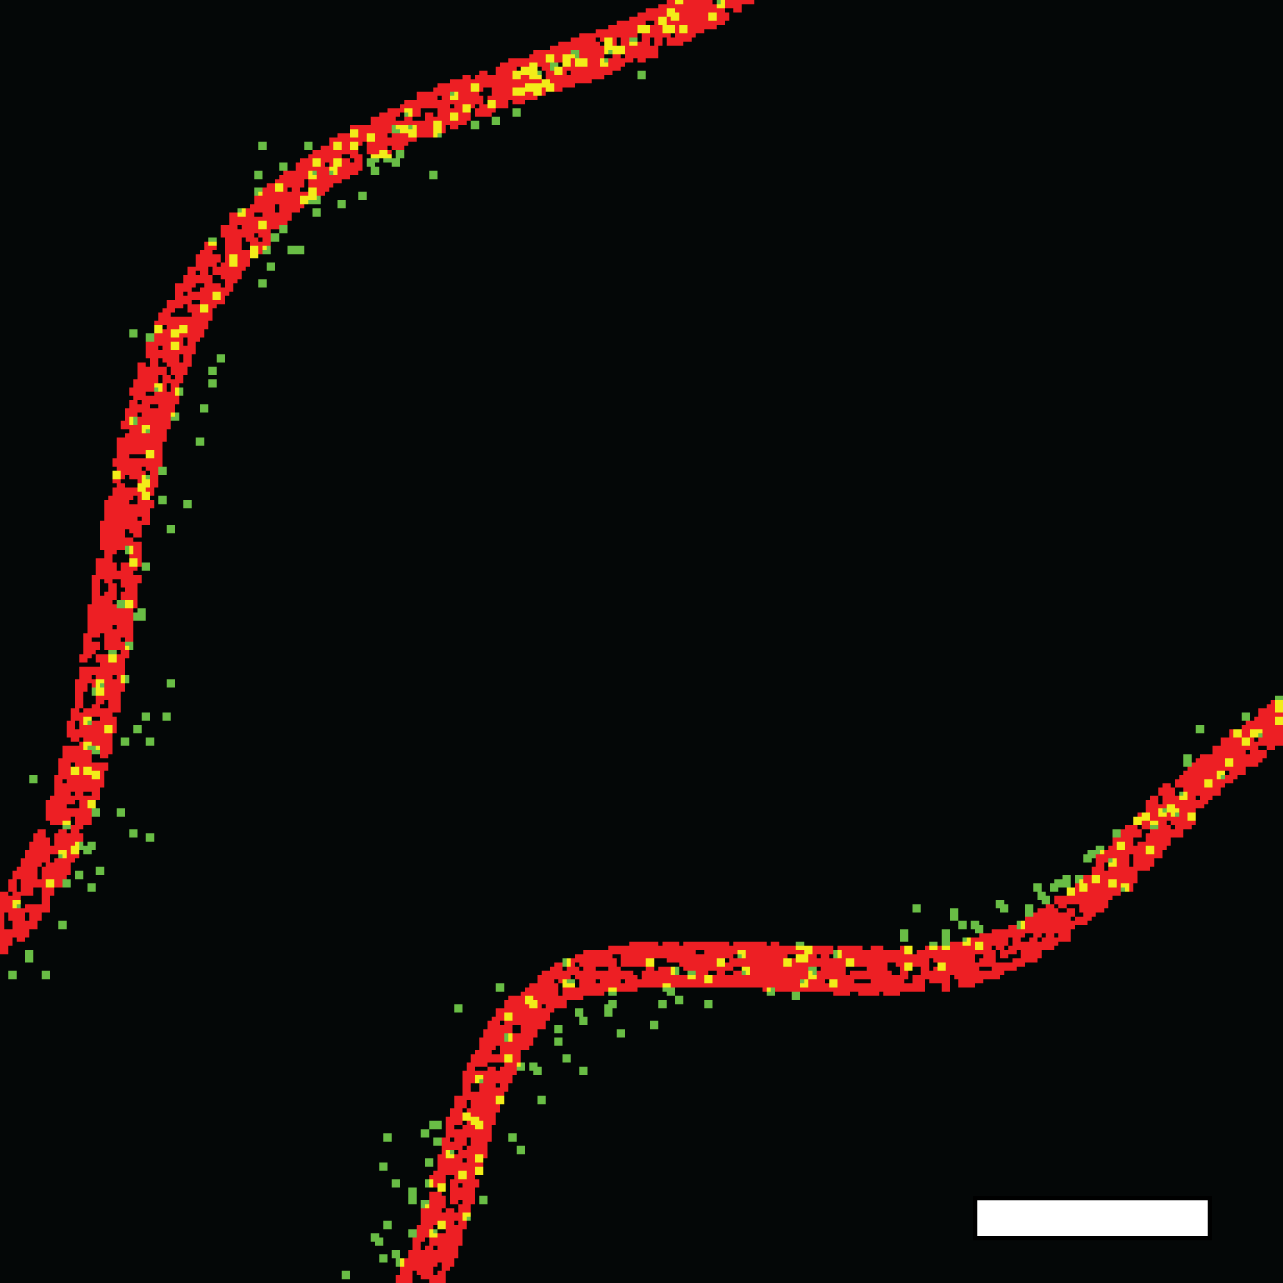
\includegraphics[width=0.3\textwidth]{figures/highdensityAusschnitt_gt_scalebar.png}
\par\end{centering}

\caption{High density dataset. Left: frame 3 of the raw data. Middle: reconstructed image. Right: localizations (green) and ground truth (red). Scalebar represents $1\mu m$ for the first two images and 200\,nm for the third.}\label{highdensity}
\end{figure*}

Thus, SimpleSTORM produces good results on ``normal'' data without parameter tuning, but advanced users can adjust the settings to tailor the output to the needs of a particular experiment. Specifically, it is possible to strengthen the criteria for true positives, so that only points with high certainty and correspondingly better localization accuracy are recorded. This trade-off reduces the detection performance (Jaccard and F-score), but improves the RMSE (it is not possible to improve both at the same time). To this end, SimpleSTORM offers the opportunity to set the p-value, an asymmetry threshold and the upscaling factor for the reconstructed image. Table \ref{improvements} shows the changes in Jaccard index, F-score and RMSE for the `long sequence' dataset after these changes. Baseline settings are: $p$-value = 0.1~\%, upscaling factor = 10 and asymmetry threshold off.
\begin{table}
\caption{Effect of advanced parameter settings.}
\begin{tabular}{l|ccc}
&Jaccard&F-score&RMSE\\\hline
baseline&0.824&0.903&12.88\,nm\\
p-val = 0.001~\%&0.815&0.898&12.76\,nm\\
asymmetry (1.5)&0.620&0.765&12.13\,nm\\
upscale factor = 100&0.619&0.764&11.45\,nm
\end{tabular}
\label{improvements}
\end{table}
Lowering the p-value does not alter the results significantly, because the false positive rate is already very low. Applying an asymmetry threshold improves the RMSE, but discards a number of true positives along with the undesirable distorted spots. A higher upsampling factor increases the localization accuracy without removing any points, but increases the reconstruction time.

Finally, we also applied SimpleSTORM to real data. All images use direct stocastic optical reconstruction microscopy (dSTORM) \cite{heilemann_08_dstorm}. All three images (Figure \ref{fig:microtubuli}, \ref{fig:hela2-tubulin} and \ref{fig:hela2-actine}) were captured using a exposure time of 100~ms, a frequency of 9.8~Hz and an iradiation intensity of 3.5 kW per square cm. A qualitative impression is given in figures \ref{fig:microtubuli}, \ref{fig:hela2-tubulin} and \ref{fig:hela2-actine}. In figure \ref{fig:microtubuli}, we can even make a qualitative statement: the depicted microtubuli have a true diameter of about 25nm, whereas the diameter in the reconstruction is about 60nm. Considering the expected RMSE and the average distance of the fluorescent markers from the actual molecule, this is in the expected ballpark.
\begin{figure*}
\begin{centering}

\includegraphics[width=0.3\textwidth]{figures/AVG_Hela2_aTub647-i.png}$\qquad$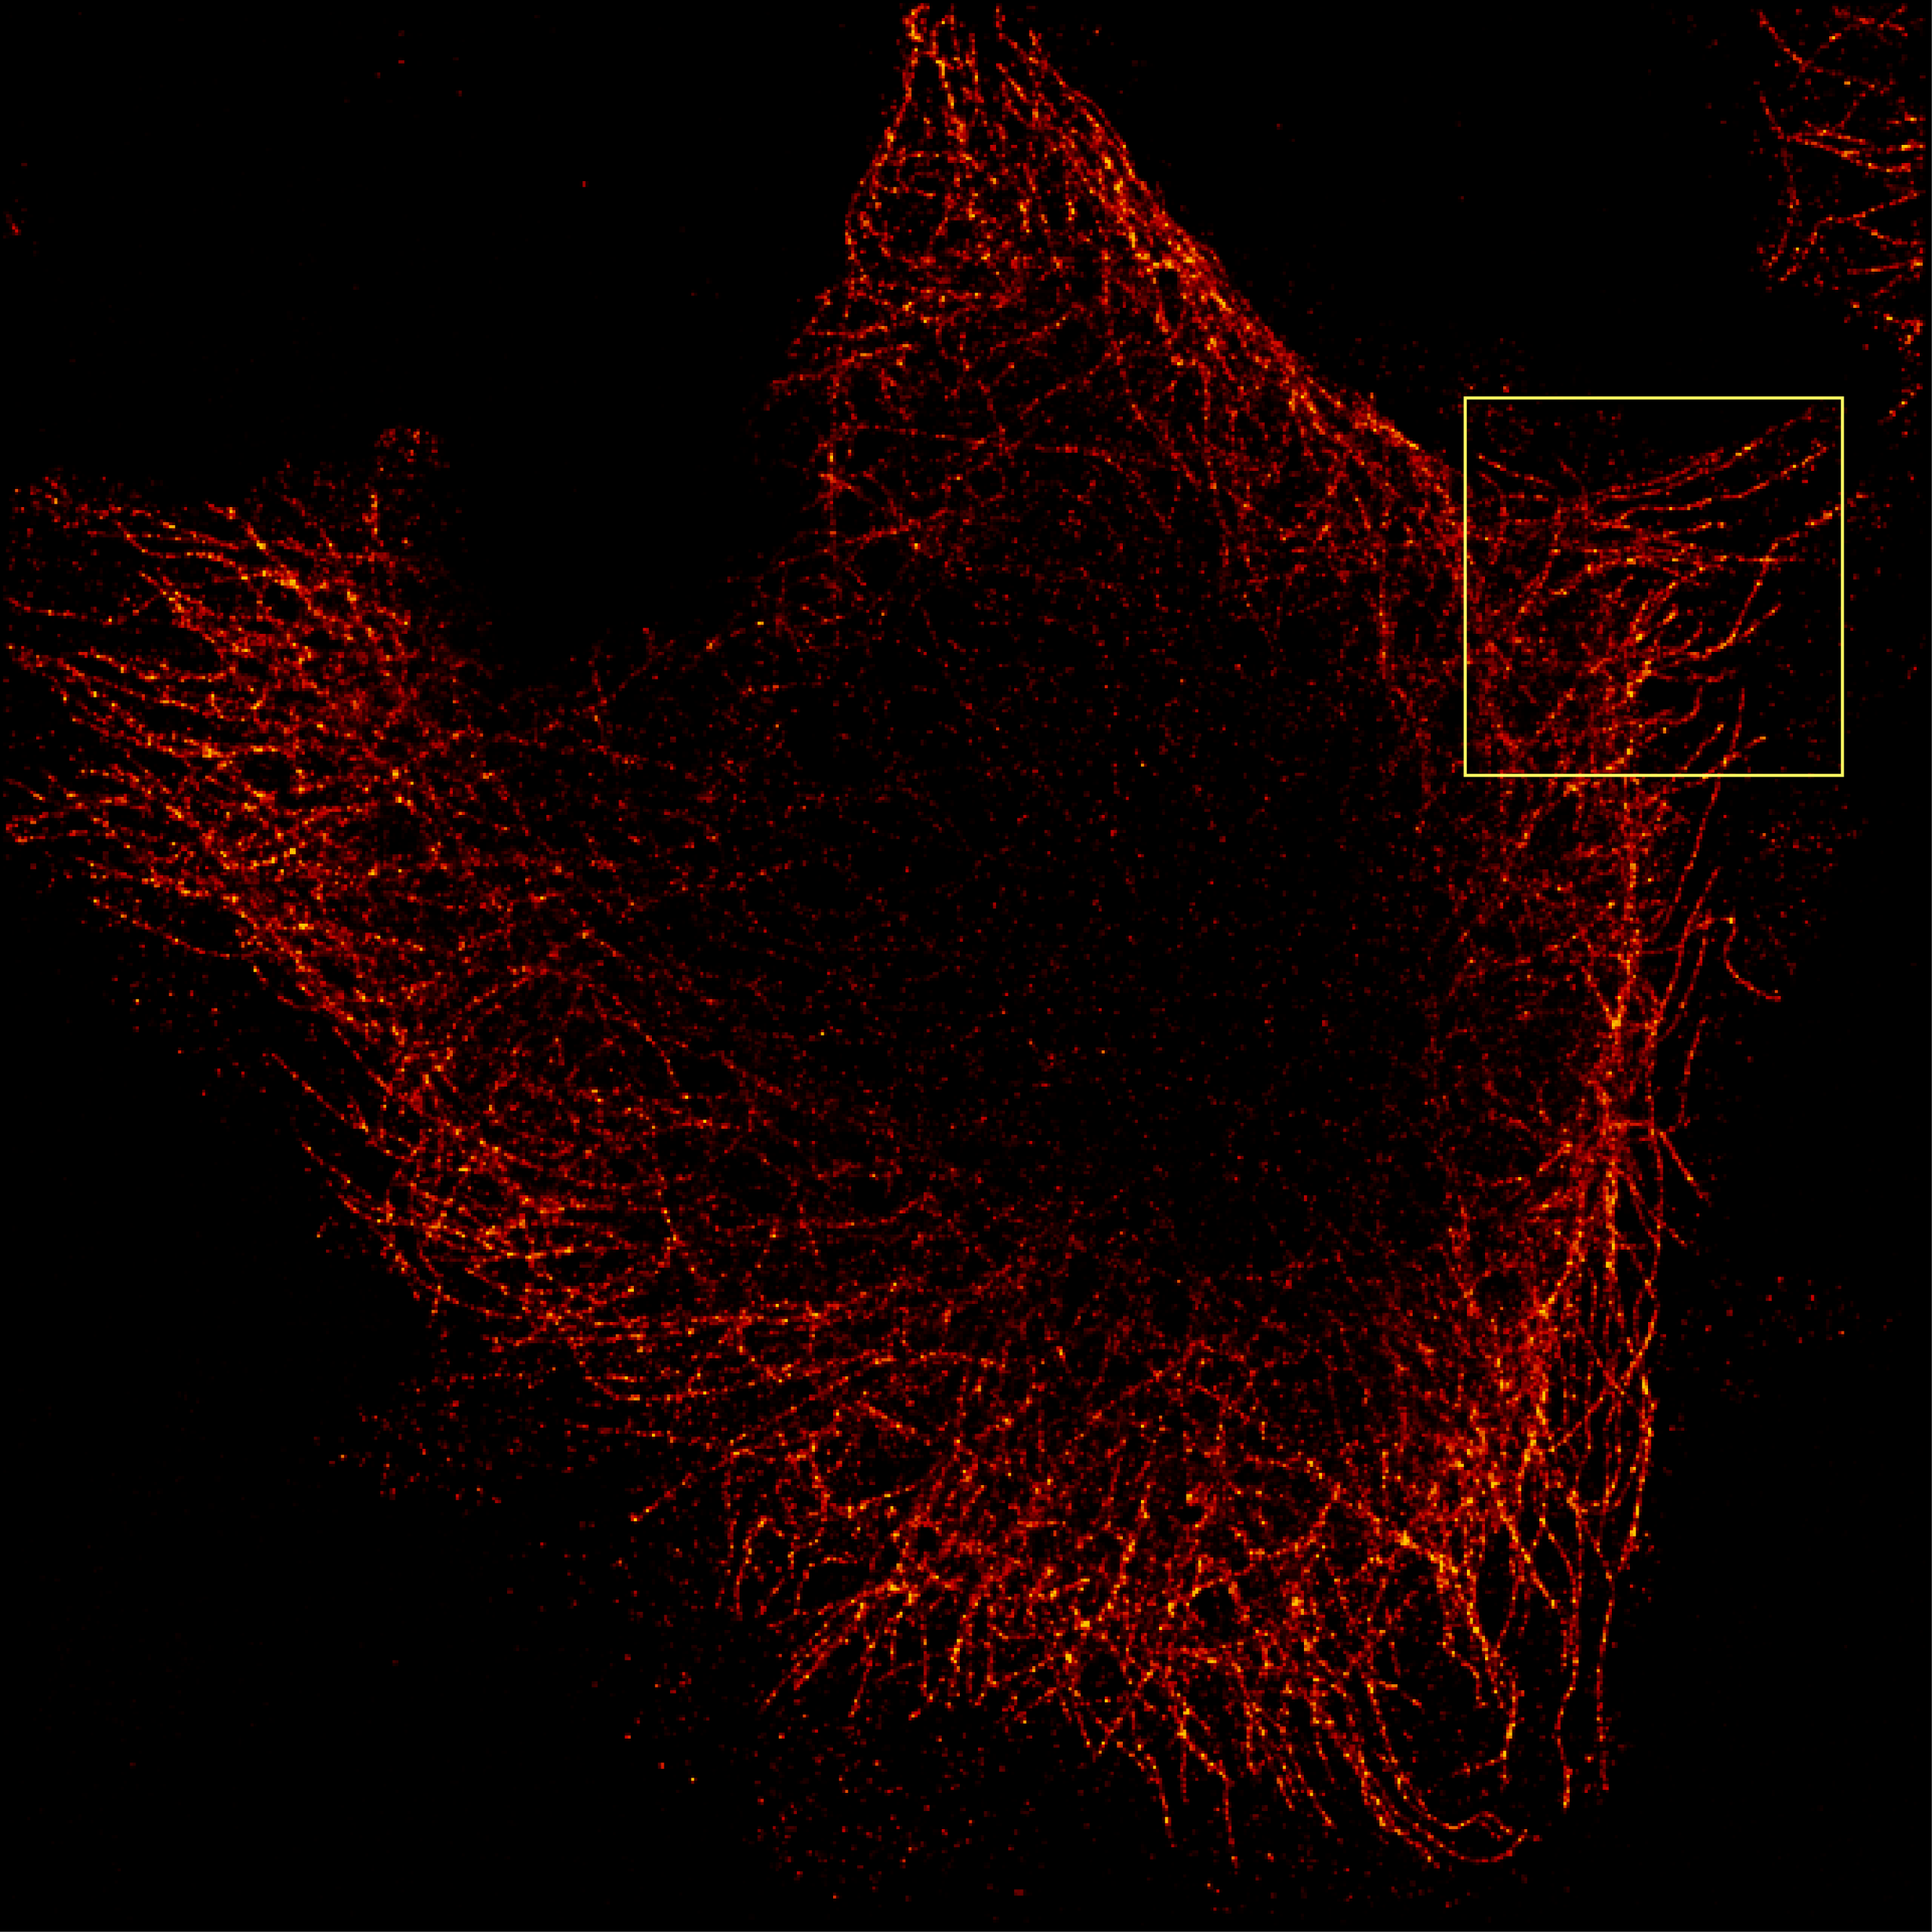
\includegraphics[width=0.3\textwidth]{figures/HeLa2_aTub647-i_resultHighContrast-1_reconstructed_rect.png}$\qquad$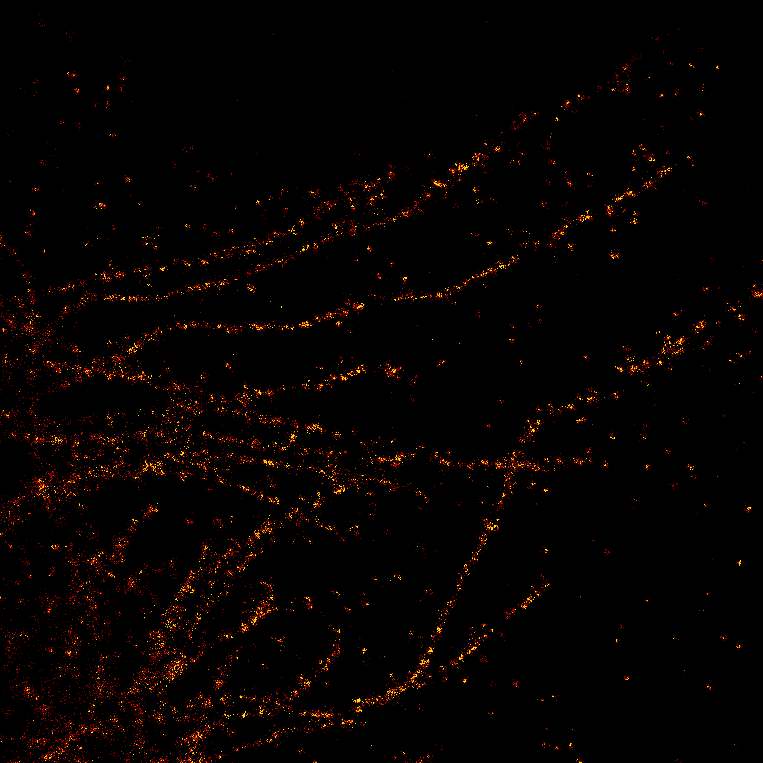
\includegraphics[width=0.3\textwidth]{figures/HeLa2_aTub647-i_resultHighContrast-1_rect.png}
\par\end{centering}

\caption{Beta-tubulin labeled with AlexaFluor647 in a Hela cell. simpleSTORM.
Left: mean image of the raw data. Middle: reconstruction by SimpleSTORM. Right: magnification of the indicated subregion.}\label{fig:hela2-tubulin}
\end{figure*}
\begin{figure*}
\begin{centering}
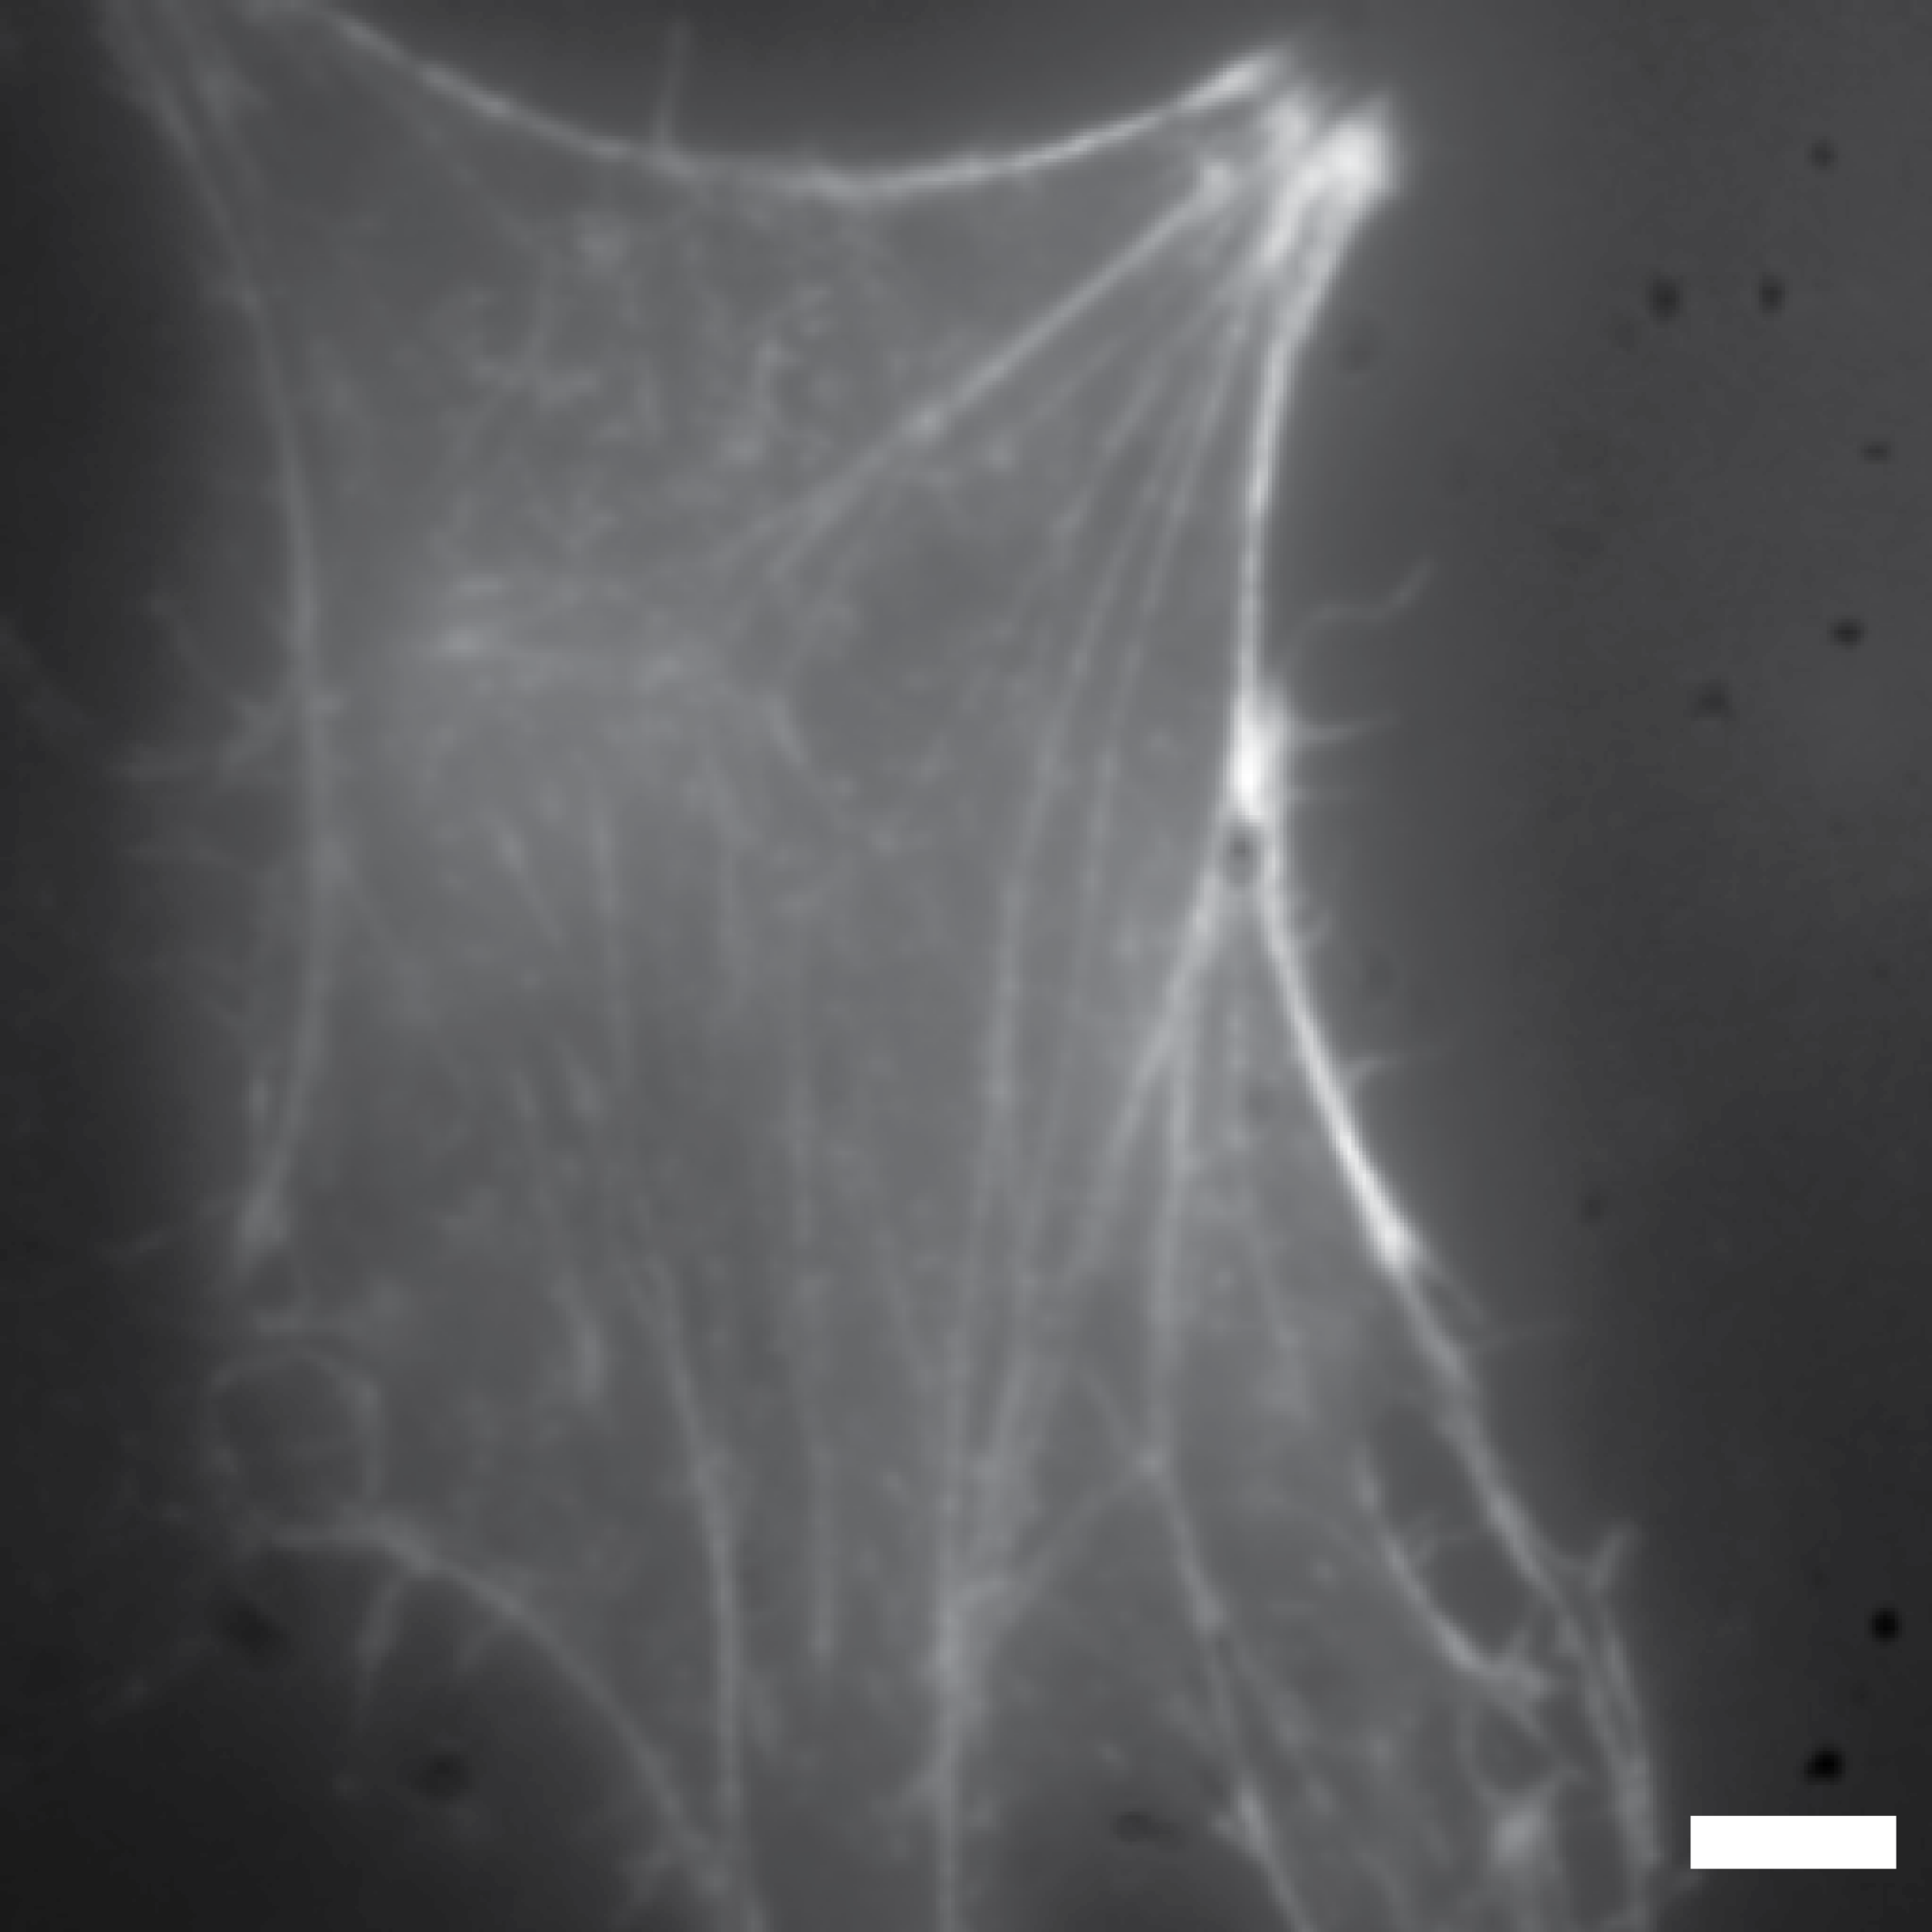
\includegraphics[width=0.45\textwidth]{figures/AVG_110603_HeLa2_actin-mEOS2-2_scalebar.png}$\qquad$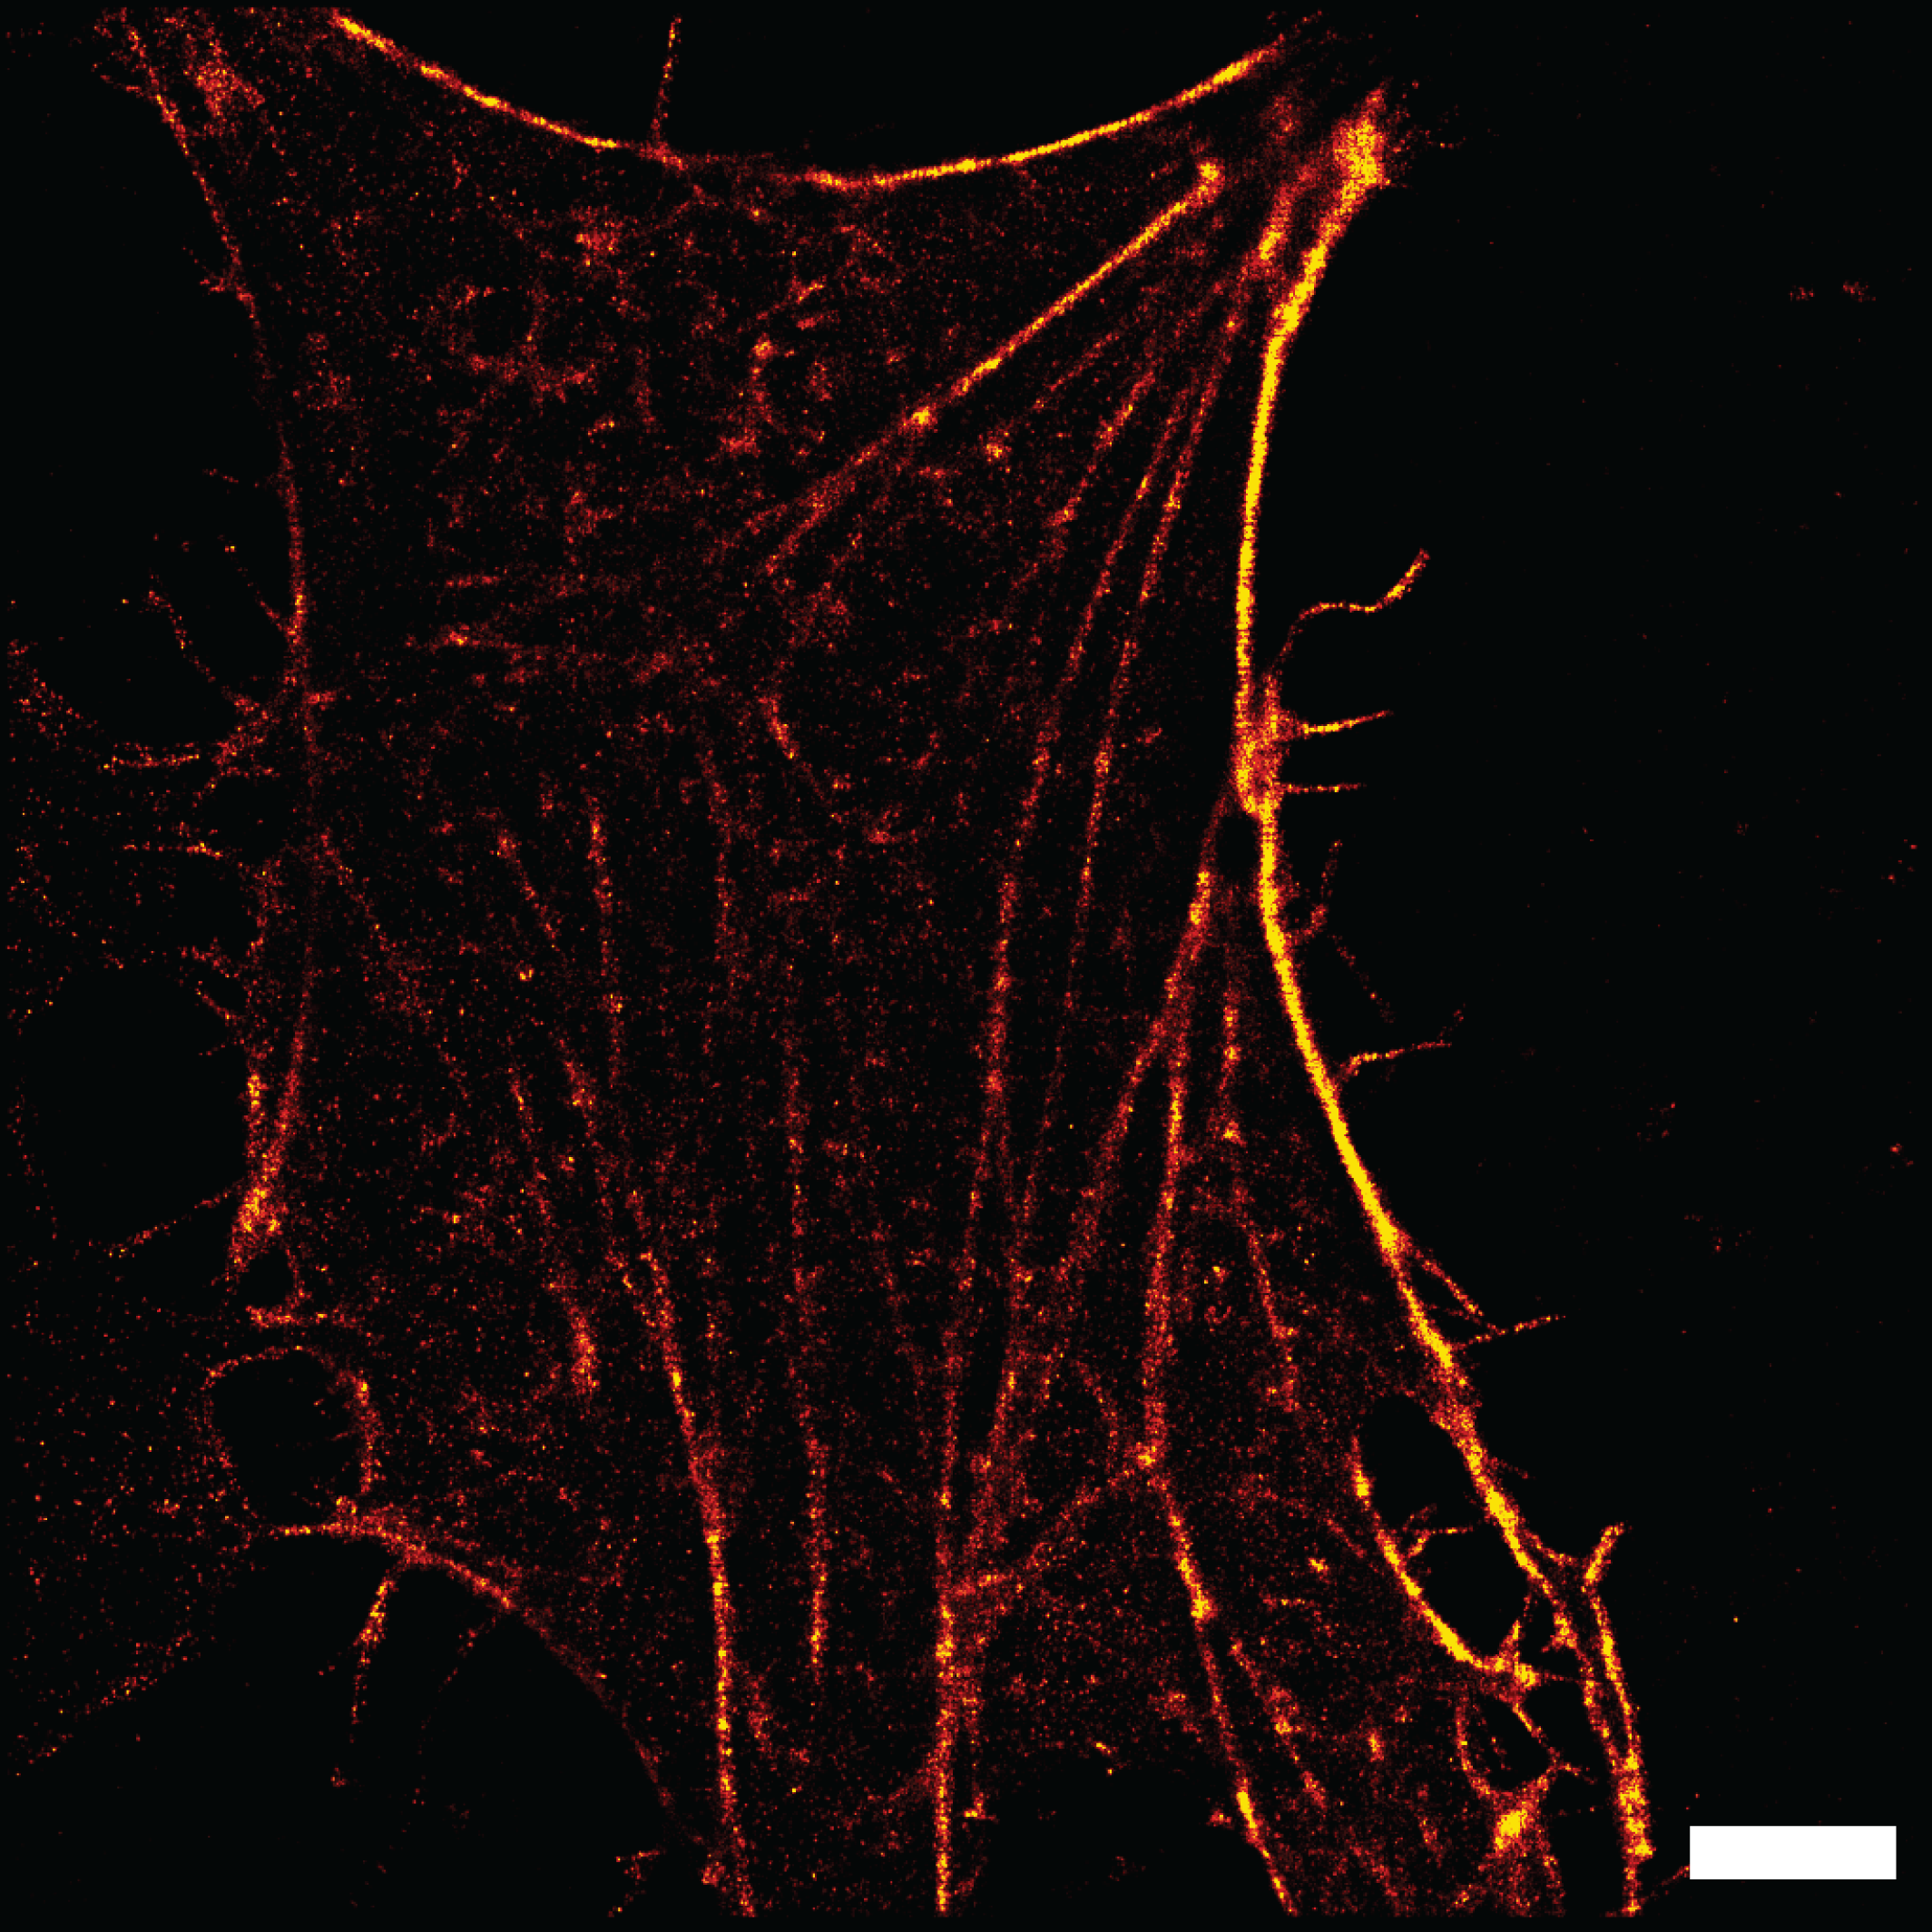
\includegraphics[width=0.45\textwidth]{figures/110603_HeLa2_actin-mEOS2_resultHighContrast-1_scalebar.png}
\par\end{centering}

\caption{Actin labeled with mEos2 in HeLa cells.
Left: mean image of the raw data. Right: reconstruction by SimpleSTORM. Scalebars represent $3\mu m$}.\label{fig:hela2-actine}
\end{figure*}


\begin{acknowledgements}
This research was supported by contract research ``Methoden f{\"u}r die Lebenswissenschaften'' of the Baden-W{\"u}r\-ttemberg Stiftung.
We are gratefull to Mike Heilemann and Benjamin Flottmann for providing the raw data of the images presented in this paper.
\end{acknowledgements}

\bibliographystyle{spbasic}
\bibliography{simpleSTORM}

\end{document}
